\documentclass[fleqn,12pt]{olplainarticle}
% Adds SVG Support out of cls file
\usepackage{svg}
% Merge multiple references into 1
\usepackage[noadjust]{cite}

% Double line spacing
% \usepackage{setspace}
% \doublespace
%\linespread{2pc}

% Fancy table related trick
\usepackage{multirow}
\usepackage{tikz}
\usepackage{makecell}
\def\chk{\tikz\fill[scale=0.4](0,.35) -- (.25,0) -- (1,.7) -- (.25,.15) -- cycle;}

% Python code
\usepackage{listings}

% Algorithmic
\usepackage{algorithm, algorithmic}

% Subfigures
\usepackage{caption}
\usepackage{subcaption}

%New colors defined below
\definecolor{codegreen}{rgb}{0,0.6,0}
\definecolor{codegray}{rgb}{0.5,0.5,0.5}
\definecolor{codepurple}{rgb}{0.58,0,0.82}
\definecolor{backcolour}{rgb}{0.95,0.95,0.92}

%Code listing style named "mystyle"
\lstdefinestyle{mystyle}{
  backgroundcolor=\color{backcolour},   commentstyle=\color{codegreen},
  keywordstyle=\color{magenta},
  numberstyle=\tiny\color{codegray},
  stringstyle=\color{codepurple},
  basicstyle=\ttfamily\footnotesize,
  breakatwhitespace=false,         
  breaklines=true,                 
  captionpos=b,                    
  keepspaces=true,                 
  numbers=left,                    
  numbersep=5pt,                  
  showspaces=false,                
  showstringspaces=false,
  showtabs=false,                  
  tabsize=2
}

%"mystyle" code listing set
\lstset{style=mystyle}

% lscape.sty Produce landscape pages in a (mainly) portrait document.
\usepackage{pdflscape}

% Adding if execution to define between thesis and article
\usepackage{ifthen}
\newboolean{thesis}
\setboolean{thesis}{false}

\title{Practical review of Lithium-Ion battery State of Charge estimation using Time-Series Machine Learning for Electric Vehicles.}

\author[1]{Mr Marat (Matt) Sadykov}
\author[2]{Asoc/Pr David Holmes}
\author[3]{Asoc/Pr Geoff Walker}
%\author[4]{\\Dr Mark Broadmeadow}

\affil[1]{Queensland University of Technology}
%\affil[2]{Address of second author}
%
% IF
\ifthenelse {\boolean{thesis}}
%
% THEN
{
\keywords{
    Adaptive Moment Estimation (Adam),
    Adaptive Moment Estimation based on the infinity norm (Adamax),
    Attention Layer,
    Chip-on-Board (CoB),
    Electric Vehicle (EV),
    Gradient Recurrent Unit (GRU),
    Lithium-Ion battery (Li-Ion),
    Long Short-Term Memory (LSTM),
    Nesterov Adaptive Moment Estimation (Nadam),
    Raspberry Pi 4 (R-Pi4),
    Recurrent Neural Networks (RNN),
    Robust Online Adaptive Moment Estimation (RoAdam),
    State of Charge (SOC) estimation,
    Stochastic Gradient Descent with Momentum (SGDw/M),
    Tensor Processing Unit (TPU),
    TensorFlow (TF),
    Time-Series Machine Learning
    }
}
%
% ELSE
{
%\keywords{Driving schedulers, Gradient Recurrent Unit (GRU), Long Short-Term Memory (LSTM), Optimisers, State of Charge (SOC) estimation, Time-Series Machine Learning}
\keywords{
    Driving schedulers,
    Optimisers,
    Recurrent Neural Networks (RNNs),
    State of Charge (SOC) estimation,
    Time-Series Machine Learning
    }
}

\begin{abstract}
    \textbf{
    %
% IF
\ifthenelse {\boolean{thesis}}
%
% THEN
{
State of Charge (SoC) estimation is critical for battery management in any battery-based electrical system.
It acts as a criterion, which justifies the amount of energy left in a single or pack of cells and how long they can supply power, for example, the endurance of electric vehicles before subsequent charging.
The ability to estimate a correct SoC and manage consumption accordingly, not only to prolong the time between charges but also the general health of the battery, in the long run, became vital for any electrical grid.
The most common way of estimating batteries charge without direct physical intervention is battery modelling.
It is possible to simulate battery behaviour by defining specific constant parameters like internal resistance and capacitance and training over sensory data of battery voltage and current consumption.
However, while some methods reasonably estimate the charge percentage, the battery losses created by Coulombic efficiency can create unpredictable behaviour with different impacts.
The Machine Learning models tend to estimate parameters themselves through the long process of training based on statistical data of battery utilization, rather than constant definitions.
The Recurrent Neural Network (RNN) treats Coulombic efficiency as part of the system by considering a short period of samples rather than single readings.
Since the wide usage of Machine Learning in many applications, there have been multiple attempts to estimate the State of Charge using Neural Nets with battery sensory data, such as Voltage, Current and Temperature.
Those methods attempted multiple model training techniques to minimize the discrepancy in available readings caused by general sensory inaccuracy and develop the best possible SoC estimator, derived from Coulomb Counting with battery testing machine.
Although it does not match actual Electric Vehicle driving, the technique validation methodology makes a reasonable way of evaluating the most efficient and low-resource consuming method.
Through the long process of critical analyses, implementation, review and comparison of the already published RNN models over multiple drive cycles, the most promising methods ended up being a Stateless model with an approximate 5-minute long history of samples, trained on LSTM model with robust adaptive Online gradient learning algorithm (RoAdam) as optimizer.
The Root Mean Squared accuracy of such models tends to be around 3.64\% against the datasets, which were not involved in the training process.
All models went through a cross-validation process over multiple datasets, and some were tested on a few embedded solutions, which can be integrated into electrical circuitry of any type.
As a result of the research, several weaknesses have been identified during reviews, such as incorrect or inefficient weight distribution across input parameters and lack of accuracy as opposed to general RNN models in other scenarios.
}
%
% ELSE
{
% \begin{itemize}
%     \item Intro statement (Application of State of Charge or Batteries)
%     \item What SoC stands for?
%     \item What or how it has been done already?
%     \item In the present paper - Investigate best ML method as a replacement to already existing ones.
%     \item How is it going to be conducted. (2-3 sentences).
%     \item What was the final conclusion or finding. That neither of them are effective and further investigation is required to be certain of safety usage inside a car.
% \end{itemize}
State of Charge (SoC) estimation is a crucial property of a Lithium-Ion battery in any electrical system.
An accurate charge percentage, without any discrepancies, allows a battery management system (BMS) to enhance battery module utilisation further, allowing higher endurance or prolonging overall utilisation for more cycles.
There have been numerous attempts to determine SoC without physical intervention, such as battery modelling.
Since batteries commonly have non-linear characteristics, statistical-based Machine Learning methods have the potential to replace the traditional model.
The present paper conducts a practical usability investigation on Recurrent Neural Networks (RNN) to determine the best-suited machine learning method for Electric vehicles (EV).
Through the implementation of models from multiple published sources and cross-validation testing with several driving scenarios of Lithium-Ion batteries, several models have been assessed on accuracy and drawbacks.% against simulations of different driving conditions.
\textcolor{red}{Each method will be examined by applied techniques, highlighting implementation and attempts to implement from the available framework as close as possible to the source with available battery data.}
The results highlight the percentage accuracy in the average of 3.64\% of Root Mean Squared Error, several drawbacks of the overall implementation and propose potential solutions for further improvement.
Every implemented model had a similar drawback of poor capturing of the middle area of a charge, applying higher weight on a voltage rather than current.
The combined techniques in a single custom model could be better suited to improve accuracy further.
}
    }
\end{abstract}

\begin{document}

\flushbottom
\maketitle
\thispagestyle{empty}
%%% Introduction
\section{Introduction} \label{sec:Introduction}
\IEEEPARstart{T}{he} market for Electrical Vehicles (EV) has grown significantly over the past decade~\cite{state-ev-australia}.
The replacement of a fossil fuel-based engine with an electric drivetrain eliminates exhaust emissions with the potential to reduce human impact on climate change significantly.
For EVs to grow market share and reduce costs, battery cost and longevity must be improved.
Extensive battery cycling leads to battery degradation over time (aging).
The development of smarter and more accurate battery management strategies may be capable of prolonging service duty.
This would rely upon a system's ability to estimate a battery's state at any point in time.
An accurate charge calculation avoids overcharging or over-discharging, leading to improved battery service utilisation, better health estimation, longer life span, more reliable range prediction and further benefits~\cite{calif_proper_2008}.

%
%
The development of effective methods for State-of-Charge (SoC) estimation remains a topic of crucial research focus.
Various techniques to estimate the SoC have been developed to enhance battery usage.
The ability to determine the state of a battery or a battery system is a required function for an advanced Battery Management System (BMS).
Those techniques can be classified into three primary categories~\cite{ali_towards_2019,ng_enhanced_2009,robust_SoC,6953745}: direct measurement, model-based methods, and computer intelligence or Machine Learning (ML).
Direct measurements methods take readings from batteries relying on sensors, such as open circuit Voltage, internal resistance, or current readings over set periods (i.e. Coulomb Counting)~\cite{ng_enhanced_2009,robust_SoC}.
Model-based methods recreate battery behaviour and use sensor inputs to calculate results from a pre-defined model~\cite{6953745}.
Computer intelligence techniques enhance such models with additional data.
Those data-driven calculations aim to improve model estimation by fitting to an actual behaviour observation.
Examples include Fuzzy Logic~\cite{malkhandi_fuzzy_2006}, Support Vector Machine~\cite{hansen_support_2005, anton_battery_2013}, or Neural Networks (NN)~\cite{song_lithium-ion_2018,Chemali2017,mamo_long_2020,jiao_gru-rnn_2020,xiao_accurate_2019,javid_adaptive_2020,zhang_deep_2020}.

%
%
While some model-based methods, such as the equivalent circuit model, are simple to implement within a BMS, many cannot correctly capture batteries' complex multi-dependant behaviour~\cite{6953745}.
%Others are limited to offline simulation due to high complexity and computation requirements, therefore not suited to an onboard BMS.
Direct measurement estimation is limited to sensor accuracy and affected by losses created by Coulombic efficiencies~\cite{Smith_2010} where some portion of charge gets transferred to heat or gets affected by battery ageing that is not captured.
%Additionally, the measured voltage depends on whether the battery is in use or has been on rest for a given time.
%An accurate SoC estimation model has to implement a way to accommodate battery losses and sensor readings.
%If model-based methods treat as constant values, then in real scenarios, they can be significantly limited to sensor inaccuracy, environmental and internal battery temperature, or aging.
%In contrast, Neural Network methods can accommodate losses as they can capture complex phenomenological behaviours~\cite{bengio_learning_1994}.
%
%Smart BMSs, which incorporate some method of ML, use only sensory data~\cite{zhang_deep_2020} and do not require a batteries physical property~\cite{zhang_deep_2020}.
In contrast, Machine Learning are known to be able to establish relationships in complicated and multi-dimensional non-linear systems~\cite{hansen_support_2005,anton_battery_2013,he_state_2014}.
This characteristic shows great potential to account for battery losses due to Coulumbic efficiency.
Some researchers used the support vector machine-based methods to estimate SoC using voltage, current, and temperature inputs~\cite{hansen_support_2005,anton_battery_2013}.
Data were obtained from a driving schedule profile on a battery cycler, and the end error estimation was achieved as less than 6\%~\cite{he_state_2014}.
%The solution to lowering that percentage may lie within the more complicated models, like Neural Networks.
Many attempts to implement different Neural Networks exist, but the most promising net for charge estimation were Recurrent Neural Networks (RNN)~\cite{song_lithium-ion_2018,Chemali2017,mamo_long_2020,jiao_gru-rnn_2020,xiao_accurate_2019,javid_adaptive_2020,zhang_deep_2020}.
Their effectiveness in time-series dependant problems was shown using internal neurons to process data sequences with varying lengths by Chemali et al.~\cite{Chemali2017}.
% The models' cells act as memory units, building relationships and giving outputs based on multiple inputs over time.
% Typical examples are data forecasting, handwriting, speech and image recognition, machine translation or music composition~\cite{devdarshan_applications_2019}. 

% 
%
Over the past years, the RNN approach has found multiple applications for SoC estimation.
The most recent attempt to determine the Li-Ion battery's remaining useful life was with implementation of the Gradient Recurrent Unit models~\cite{song_lithium-ion_2018,javid_adaptive_2020,xiao_accurate_2019,jiao_gru-rnn_2020}.
The earliest approach utilised a battery charge's regression nature only using stateless models~\cite{song_lithium-ion_2018,jiao_gru-rnn_2020,xiao_accurate_2019} when input impact is not preserved for further predictions.
Later, some approaches introduced additional parameters to support the NN learning process~\cite{mamo_long_2020,jiao_gru-rnn_2020,javid_adaptive_2020}.
Besides good convergences, the model's use was in determining critical events, like the time before complete charge depletion or overcharge.
However, it did not receive wide application due to its initial state requirement as input features.
The most popular way lies in determining the charge's value using a fixed size history of voltage, current, and temperature in stateless Long Short-Term Memory (LSTM) models~\cite{Chemali2017,mamo_long_2020,javid_adaptive_2020,zhang_deep_2020}.
The method's advantage is independent of the charge or discharge cycles at different times, as long as the history samples are in order.
However, estimation determines values based on fixed history samples and does not preserve for the next prediction, making practical estimation of single or several charge values, but not determining critical events ahead.
That can be achieved with stateful models, which continuously preserve the prediction's impact and can be propagated further until they reach the end state without resets~\cite{zhu_statefulnes_tfdocs_2020}.

%
%
One of the first attempts to train an RNN model to predict the state of charge is to train in several cycles of a single battery utilisation dataset at different temperatures~\cite{song_lithium-ion_2018, xiao_accurate_2019,javid_adaptive_2020, jiao_gru-rnn_2020}.
Then as others attempted to generalise battery behaviour to multiple usage scenarios, which as comparison lead to higher Root Mean Squared Error.~\cite{mamo_long_2020}.
For instance, by comparing similar procedures of testing from Song et al.~\cite{song_lithium-ion_2018} and Mamo et al.~\cite{mamo_long_2020} who conducted their research methods but used different validation mechanisms, it can be seen how accuracy error doubles if testing performs at a different temperature or untrained driving profile.
By selecting same drive cycles at closely similar temperature, Song et al.~\cite{song_lithium-ion_2018} accuracy acchieved rougly 0.735\% error, then as Mamo et al.~\cite{mamo_long_2020} reported 1.2533\% at best.
This can be explained that most researchers used a single driving profile, but with an entire available temperature range for training and then a portion of handpicked temperatures for validation and accuracy report.
This behaviour is less realistic to the actual scenario since during a single acceleration event, the battery goes through ambient temperature to the maximum allowed within several seconds, and its' usage depends on the condition of a road and drivers experience.
Mamo et al.~\cite{mamo_long_2020} attempted to generalise this behaviour by using the addition layer construction technique to make a model be appliable to any driving condition and more realistic scenario.
There has been little research to validate the performance of different Machine Learning techniques to extrapolate ideal laboratory batter cycling conditions of early collected data to an electric vehicle behaviour.
%% (Include to one of the sections)
% After identifying the most optimal input preferences without significant effect on the performance, one of the further developments apply changes to the structure of GRU or LSTM by adding additional layers (Attention or Extra Dense layers)~\cite{mamo_long_2020, jiao_gru-rnn_2020}.
% Another way is to change the optimisation process to achieve similar accuracy faster (i. e., adding a Momentum algorithm to the Stochastic Gradient Optimisations process or replacing gradient calculations with statistical)~\cite{xiao_accurate_2019, javid_adaptive_2020}.
% Those methods modify standard ways introduced earlier in model training by applying additional operations.
% As a result, they met to achieve better accuracy faster using similar training approaches. 
However, after identifying the most optimal input preferences, some researchers applied changes to the structure of models by adding additional layers (Attention or Extra Dense layers~\cite{mamo_long_2020, jiao_gru-rnn_2020}) or modified optimisers (i. e., adding a Momentum algorithm to the Stochastic Gradient Optimisations process~\cite{xiao_accurate_2019}) to further enhance the speed of the training process to achieve the lowest error.
\mbox{Table~\ref{tab:review}} summarises the most common methods applied to SoC estimation, highlighting the model cell type, structure to define input sample type, optimiser selection, and additional features introduced by authors to improve predictions.
\textcolor{red}{\textbf{Matt: I moved most of the details about the table to caption. However, since this paragraph and next were swapped I had to do my best to avoid driving profile mentioning where possible. Perhaps we should consider swapping them back or some sentences.}}
\begin{table*}[h]
    \renewcommand{\arraystretch}{1.3}
    \caption{Reviewed papers implementation summary.
    The model type highlights a primary path in structuring a Neural Network.
    The statefulness defines the input method, where stateless uses a fixed size of input samples per each feature and statefully apply each time sample at a time for all features one by one.
    %Optimiser selection sets the algorithm for the learning process from one of the following methods: Adaptive moment estimation (Adam), Nesterov adaptive moment estimation  (Nadam), Stochastic gradient descent (SGD), AdaMax (AM) and Differential Evolution (DE).
    Optimiser defined from: Adaptive moment estimation (Adam), Nesterov adaptive moment estimation  (Nadam), Stochastic gradient descent (SGD), AdaMax (AM) and Differential Evolution (DE).
    }
    \centering
    \label{tab:review}
\resizebox{\textwidth}{!}{
\begin{tabular}{l|c|c|c|c|c|c|c|c|c|l}
    \hline\hline \\[-4mm]
    \multicolumn{1}{ c }{} & 
    \multicolumn{2}{|c|}{Model} & 
    \multicolumn{2}{ c|}{State-} & 
    \multicolumn{5}{ c|}{Optimiser} &
    \multirow{2}{ 4em }{Extension} \\
    \cline{1-4} \cline{5-10}
    Reference source & GRU  & LSTM & -less & -ful & Adam & Nadam & SGD & AdaMax & DE\footnote{Differential Evolution} & \\
    \hline
    Song~\cite{song_lithium-ion_2018}
        & \chk &      &      & \chk & \chk &      &      &      &      & 4 Layers  \\
    Chemali~\cite{Chemali2017}
        &      & \chk & \chk &      & \chk &      &      &      &      &           \\
    Mamo~\cite{mamo_long_2020}
        &      & \chk & \chk &      &      &      &      &      & \chk & Attention \\
    Jiao~\cite{jiao_gru-rnn_2020}
        & \chk &      &      & \chk &      &      & \chk &      &      & Momentum  \\
    Xiao~\cite{xiao_accurate_2019}
        & \chk &      &      & \chk &      & \chk &      & \chk &      & Ensemble  \\
    Javid~\cite{javid_adaptive_2020}
        & \chk &      & \chk &      & \chk &      &      &      &      & Robust    \\
    Zhang~\cite{zhang_deep_2020}
        &      & \chk & \chk &      &      & \chk &      &      &      & Online    \\
    \hline\hline
\end{tabular}
}
\end{table*}

% Althpugh, experement which involved extrapolation ideal laboratory conditions with accurate sensory to a real world conditions, woth different environmental charecteristic or sensorary interferance - is not currently available.
%
In most published testing of ML methods applied to SoC, experiments on battery cycling data were conducted on different cell types.
Most used table data of real-time sensory results from battery cyclers to validate efficiencies generated using different current schedulers (driving profiles)~\cite{Chemali2017,song_lithium-ion_2018,mamo_long_2020,jiao_gru-rnn_2020,xiao_accurate_2019}.
%An equally time-based sample of current consumption acts as an input to the battery cycler, intended to recreate a stress test on a battery or human driving behaviour.
There are three the most commonly used in the research of this area: Dynamic Stress Test (DST) for a variable power discharge mode, aggressive Highway Drive Schedule (US06) and Federal-Urban Driving Scheduler (FUDS) for nominal driving scenarios.
Unlike some general simple static discharge processes, which commonly appear in other battery-based tools, driving profiles include some amount of regenerative driving to simulate the actual application of the battery for an electric vehicle.
%
% Mamo et al.~\cite{mamo_long_2020} conducted experiments by validating the RNN model performance by training one driving profile and testing against the other two.
% The results showed doubled higher Root Mean Squared Error, as opposed to training and validation over single driving profiles as per experiments by Xiao et al.~\cite{xiao_accurate_2019}.
%
The process of identifying the best-suited method for a specific condition, like driving an EV, is one of the crucial steps for machine learning engineering.
It requires carefully defined methodology, which characterises researched conditions as close as possible, and experimental results from multiple models with appliable techniques and the lowest errors.
By comparing implementation and results from different sources and testing accuracy and performance against multiple driving conditions at various temperatures from ambient to maximum possible, it is possible to select the best machine learning technique, which can be integrated directly into an Electric vehicle and safely used either on tight city roads or long high-speed highways.
%There have not been many similar experiments against other SoC estimation methods since such validation procedures are necessary for the computer intelligence method compared to battery modelling.
% In addition, all investigations did poor research in extrapolating ideal laboratory conditions with battery cycler, stable temperatures and no sensor discrepancies to an actual driving situation on the road, mainly due to lack of car data.
%
% Usage of a single profile's battery cycling data may not validate ML methods' efficiency in driving an electric vehicle.
% The inability to determine the charge's current state during EV driving makes the online learning process inapplicable.
% Even with other SoC estimation technique usage, the computational complexity of training any NN is complicated to fit on a low power device.
% An offline trained model had the advantage of insignificant resource consumption during the prediction stage, making it a prefered way for an EV.
% All further model testing will be applied through varying battery cycling profiles to capture the influence of data type to model efficiency.
%
% (No point)
% The drawback lies within the validation procedures of produced models.
% Ideally, this process must be performed with similar data but under different conditions or at different times.
% However, once the produced model is taken through different unseen scenarios, the accuracy lowers drastically compared to early reported results since it starts to experience something completely unexpected.
% The lack of training samples or means to produce at different conditions affected the final judgment results of many publications. 
% Even though the estimation produces accurate output with tabled data, placed under actual driving conditions - the model will have difficulties matching training performance. 


%
%
% Mamo et al. conducted experiments
%
% ------------------------------------------------------------------------ \\
% PAPER CONTRIBUTION may be worth adding as a clear statement \\
% ------------------------------------------------------------------------ \\
% Asses handpicked articles from different categories of SoC estimation, asses efficiency and complexity to utilise in EV.
% This paper's contribution lies in researching recent approaches used to estimate Charge's State from battery sensor readings.
% Comparing and implementing the most promising algorithms intended to determine the direction to build upon in the future. \\ \\
% This paper will test recent developments in the most common SoC prediction to determine the most promising direction/approach towards implementing an improved and light model applied to an electric vehicle.
% It determined to find the ML model creation's weakness and implement a new one for an EV. \\
% ------------------------------------------------------------------------ \\
%
%
% This paper investigates, implements and compares extended memory-based models of RNN to predict the State of Charge and additional built-on over time techniques to select the most effective and least resource requiring onboard-based computations appliable within Electrical Vehicles.
This paper investigates, implements and compares extended memory-based models of RNN to predict the State of Charge and additional built-on over time techniques to select the most suitable for practical application to be used in EV using combinations of different profiles.
Each subset will contain implementation from various articles changing either structure of the models or learning approaches.
It should help develop a methodology that will be further used to extrapolate offline trained methods from the lab condition to the road drive tests.
% The recent advancement and commonly used subsets are Gradient Recurrent Unit and Long Shot-Term Memory unit cells.
% Recurrent Neural Network has been confirmed to be suitable for the battery-related system by authors discussed further, such as Chemali~\cite{LSTM_Hochreiter1997}.
% However, there is no valid proof of if GRU or LSTM is helpful for battery SoC estimation.
% The best way to separate them and explore differences and efficiencies is to use them as Stateful and Stateless models.
The A123 Lithium-Ion battery data with three typical driving profiles, obtained from the University of Maryland 2012~\cite{noauthor_calce_2017} cycling experiment will act as training and testing samples.
Each method will be validated through those samples (either DST, US06 or FUDS driving profiles) and tested against robustness and accuracy of estimation of State of Charge of batteries in the other two unseen schedulers.
%
The remaining sections are organised as follows: all methodology with details regarding training procedure outlined in Section~\ref{sec:Meth}, with processing data in Subsection~\ref{subsec:b_data} and testing hardware in Subsection~\ref{subsec:soft}.
Every detail on algorithms and optimisers are written in Section~\ref{sec:Body}, where Subsection~\ref{subsec:structure} separates all details for each GRU and LSTM method, and Subsection~\ref{subsec:optimisers} breaks down every applied optimising algorithm.
Section~\ref{sec:conclussion} gives the results of implementation, performance characteristics and concludes the critical analysis.

%%% Body
\section{Time-series models implementation} \label{sec:Body}
This section focuses on a detailed overview of each component required to build and train the Machine Learning model.
It will go through each type of model used in this investigation and breaks them part by part to overview potential strengths and weaknesses.
In addition, every optimiser will be discussed in the growing complexity order to visualise their development process over time and pick the most processing for the final goal.
Classical RNN consists primarily of three layers, represented in \mbox{Figure~\ref{fig:RNN-structure}}.
\begin{figure}[htbp]
    \centering
    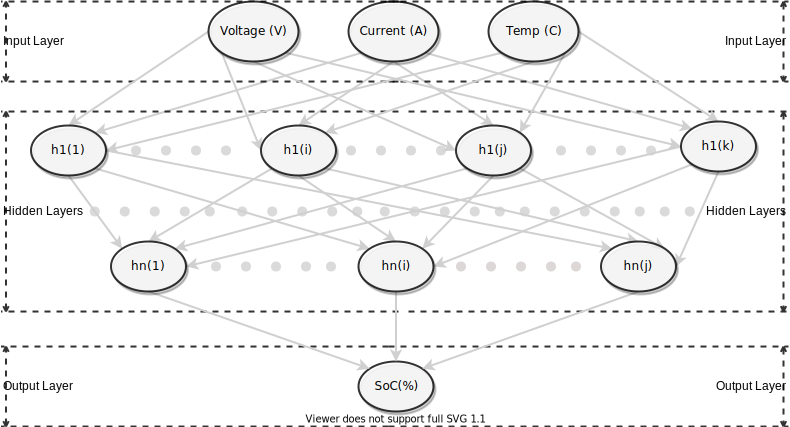
\includegraphics[width=\columnwidth]{II_Body/images/SoC-RNN.png}
    \caption{Universal structure of RNN for SoC estimation.}
    \label{fig:RNN-structure}
\end{figure}
%
%   Model Structure
%
\subsection{Model structure} \label{subsec:structure}
The general summary model structure is represented in \mbox{Figure~\ref{fig:RNN-structure}}, with three feature inputs and a single output.
The number of hidden layers will be dependant on the authors' implementation.
Since the output consists of only a single sample, it is defined by a fully connected layer - a dense layer with a single neuron.
In case if the article did not specify the number of neurons per layer, the following equations have been used to get the initial raw estimation~\cite{eckhardt_choosing_2018}:
\begin{equation}
    \begin{split}
        N_h &= \frac{N_s}{ a \left(N_i+N_o \right)} \ \ OR \ \ N_h = \frac{2}{3}\left(N_i+N_o \right) \\
        N_i &\rightarrow \text{Number of input neurons} \\
        N_o &\rightarrow \text{Number of output neurons} \\
        N_s &\rightarrow \text{Number of samples in training data set} \\
        \alpha &\rightarrow \text{An arbitrary scaling factor 2(5)-10}
    \end{split}
\end{equation}
%**Contrary with Hidden Layers as per their name, they obey only internally defined logic and connections.
%**That is why models are stable and reliable once created, cannot be changed, only retrainable with different data.
%A standard Hidden layer, consisting of fully connected neurons, called a Dense Layer.
%A standard Hidden layer, consisting of fully connected neurons and only one or none activation function, called a Dense Layer.
%Within each cell of a Dense layer lies a single activation function.

%An Output Layer gets created from Dense Layer and commonly with no Activation function.
%: \textit{Simple, Exponential or Rectified Linear; Sigmoid and Hyperbolic Tangent functions}. \\
% \begin{itemize}
%     \item \textit{linear} - Simple Linear function
%     \item \textit{elu} - Exponential Linear function
%     \item \textit{relu} - Rectified Linear unit function
%     \item \textit{sigmoind} - Sigmoid function $sigmoid(x) = 1/1(1+exp(-x)$
%     \item \textit{tanh} - Hyperbolic Tangent function $$
% \end{itemize}

%
%
There are several activation functions for those layers widely used in machine learning libraries for time series problems~\cite{amidi_cs_2018}.
For the SoC prediction problem, all authors used the same function.
It also was experimentally confirmed that the best one for all hidden layers is the hyperbolic tangent function, \mbox{Equation~\ref{eq:tanh}}.
The output layer does not use the same logic, and no activation gets applied.
A dropout layer technique with a 20\% cut-off has been applied to all hidden layers to prevent data overfitting over long training periods.
\begin{equation}
    tanh(x) = \frac{sinh(x)}{cosh(x)}=\frac{e^x-e^{-x}}{e^x+e^{-x}}
    \label{eq:tanh}
\end{equation}
%
%
%The common usage of the Dense layer in this paper is the Output Layer with no activation functions and a single-neuron representing a single output SoC value.
%To apply multiple different without overcomplicating neurons, multiple layers with different or the same number of neurons or activations functions are applied.
%The more Hidden layers network contains - the deeper and computationally complex a network becomes, also referred to as Deep Neural Networks. 
% Choosing the number of neurons for a first Hidden Layer does not have a golden rule.
% For this article, the following formula helps to make a good initial estimate based on Number samples, Input and Output.\\
% \textbf{Equation}\\
% A common practice is to narrow each following Neurons by two from the previous one, to make a more accurate capture.
% To avoid overfitting data, except for data normalization and Input sample shuffling in stateless models, a Dropout technique gets applied.
% Tensorflow has an internal implementation of Dropout for GRU and LSTM layers. A value of 0.2 (20\%) was applied to all RNN layers to minimize overfitting possibility.

%
% Requires editing below
The efficiency of an RNN over time series problem is defined by the ability of the neurons to store memory as an internal state.
With time, the memory of long passed samples may fade away.
The problem is called vanishing gradient when the value to update network weights shrinks as it propagates through time~\cite{rasifaghihi_predictive_2020}.
Long-term dependencies do not get captured since layers with a slight gradient do not significantly affect the system due to insufficient weight change~\cite{rasifaghihi_predictive_2020,hochreiter_vanishing_1998}.
The more complicated structures of neurons tend to solve that problem.
% The gradient is the value used to update Neural Networks’ weight.
%"Therefore, layers that get a small gradient do not learn, and they cause the network to have short-term memory."
% https://www.bioinf.jku.at/publications/older/2304.pdf
%"With gradient-based learning methods, the current error signals has to 'flow back in time' over the feedback connections to past inputs for building up adequate input storage. Long-term dependencies are hard to learn because of insufficient weight changes."

%
%
There are two commonly used Recurrent Neural Network, which utilises memory cells: Gated Recurrent Unit (GRU) and Long Short-Term Memory (LSTM) with possible extensions implemented by articles' authors.
The GRU implementation will be used as a stateful technique by preserving a state from batch to batch with a single sample at a time.
The LSTM will take a stateless approach, providing a fixed number of timestamps at a time.
%Implementation of the model based on simple RNN using multi-layer Dense(X) networks.~\cite{lees2010theoretical}
% a basic version of Recurrent Neural Network consists of fundamental layers with some amount of neurons.
% \subsubsection{Implementation}
%     The input data for a network has been created using Windowing technique, where \textbf{216k} sample of battery data, consisting of State Of Charge only, were separated on 500 sample windows.
%     As a result, the model outputs a single sample as SoC at the next Time Step. Using Tensorflow library and calculating number of Neurons using recommended formula \\
%     \textbf{THIS IS THE BEST PLACE FOR IT}. No other places suites as much.
%     The structure of the model ha\subsection{Training and Validation}

%s the following form. (Few Dense Layers+Dropount).
%     A Dropout layer has been used to prevent data overfitting. The selection of activation functions has been made through the data properties, which model has to fit in multiple trials.
% \subsubsection{Observation}
%     A simple Recurrent Neural Network has proven itself effective with simple Linear problems. However, with the battery state of charge, it cannot capture complicated features like the transition between Discharge and Charge or the process of Constant-Voltage Constant-Current charging. In applying battery utilisation inside Electrical Vehicle, this approach can be used only with some additional logic, such as Kalman Filters.
%     The best approach is to introduce more information about battery state and use a more complicated version of Time Series capable of memorising features with time, such as LSTM~\ref{sec: LSTM} and GRU~\ref{sec: GRU}.
    % The results of the prediction discussed in Section~\ref{sec:results}.
%\subsection{Stateful Gradient Recurrent Unit (GRU) Algorithms and Implementations} \label{subsec:GRU}
%\subsection{LSTM with Attention}\label{sec:lstm-attention}
LSTM and GRU models made the most comonly used implemtation of Time -series predictions. TadeleMamo2020 research was intended to determine waknesses and improve the model introducing addition techniques into the default structure of training model***. \\
THe attention mechanissm used in ... \\
THe intention was to capture ... \\
\subsection{Implementation}
    Attention layer implementation was taken from \textbf{refernece} github repositry of ....
    
Implementation of the model based on TadeleMamo 2020 as the most recent and how to implement improvement to the model to make it better. Gracefully transition idea from here to my model, it is similar.

    %  Gated Recurrent Unit
% Definition of the GRU
%
\subsubsection{Gated Recurrent Unit (GRU) based models} \label{subsub:gru}
One of the methods proposed by Cho et al.~\cite{GRU_cho_properties_2014}, which improves the behaviour of the Neural network, is Gated Recurrent Unit.
Unlike a simple Recurrent NN with a single activation function in the cells, GRU implements different logics to deal with vanishing gradient, as per \mbox{Figure~\ref{fig:GRU-cell}}.
On top of the activation function, it adds two gates related to input and propagated sequences.
The reset gate $r_t$ controls the level information, which has to be ignored.
The update gate $i_t$ controls the impact of previous information on the current status.
The gates implemented by \textit{sigmoid} \mbox{Equation~\ref{eq:sigmoid}} and gated get updated with \mbox{Equations~\ref{eq:GRU-gates}}.
Both gates are related to cell input sequence $x_t$ and the memory cell's output at last time stamp $h_{t-1}$.
%The structure of the layers is similar to a Dense network, with similar input and output layers.
%\textbf{Y. Song~\cite{song_lithium-ion_2018} considered them less complex than another variation (LSTM-RNN) due to the usage of 2 gates rather than 3.}
% \footnote{Bigger value - bigger impact}..
%Weight W and bias b will be the training elements. Bias is added to each gate to increase network flexibility.\\
\begin{figure}[ht]%[htbp]
    \centering
    \includegraphics[width=\linewidth]{II_Body/GRU/images/GRU.jpg}
    \caption{Gated Recurrent Unit Cell}
    \label{fig:GRU-cell}
\end{figure}
\begin{equation}
    \begin{split}
        f_t &= \sigma \left (W_{f} \left [h_{t-1}, x_t \right ] + b_f \right ) \\
        i_t &= \sigma \left (W_{i} \left [h_{t-1}, x_t \right ] + b_i \right )
    \end{split}
    \label{eq:GRU-gates}
\end{equation}
%The standard activation function or content of the memory gets modified with equation~\ref{eq:GRU-output}, where \textit{func} represent the activation function and $\ast$ multiplication by element.
The memory cell output $h_t$ get calculated through the early chosen activation function, $tanh$ in \mbox{Equation~\ref{eq:GRU-output}}.
The $\ast$ stand for multiplication by element.
\begin{equation}
    \begin{split}
        \hat{h_t} &= tanh \left (W_{\hat{h}} \left [f_t \ast h_{t-1}, x_t \right ] + b_{\hat{h}} \right ) \\
        h_t &= \left (1-i_t \right ) h_{t-1}+i_t \hat{h_t}
    \end{split}
    \label{eq:GRU-output}
\end{equation}
% The GRU can act both as a stateful and stateless cell for the model by implementing the model training library.
% For comparison, a Stateful cell will be used per implementation from Song et al.~\cite{song_lithium-ion_2018} and similar articles.
%
% By implementing a model training library, the GRU can act as a stateful and stateless cell for the model.
%(1) - not even count. The method proposed by Y.Song2018, Remaining Useful Life (RUL), \textcolor{red}{uses Capacity only. Nothing more. However, no one mentioned the Statefulnes of GRU models. This would be the best place to introduce it once properly figured out.} \\[2pc]
%
%
% (3) Method proposed by B.Xiao2019 enhances GRU model training with an Ensemble optimisation method.
% Instead of utilising standard Adam optimiser, it combines Nadam and Adamax by running one after another.
% For the first 1/3 training iterations (epochs), Nadam optimiser was used for model pre-training due to its' fast converging speed, then Adamax for model fine-tuning to determine the remaining parameters. \\
% The algorithms for model fitting are as follow \\
%
%
% (8) Similar to LSTM, a Gated Recurrent Unit is intended to solve the vanishing gradient problem.
%     Unlike Chemali2017 implementation, where the training set has consisted of input data sequences with stateles model, BinXio2019 used a stateful model within batches. In addition, it introduced a technique of optimisation to the speedup training process.
%     Implementation of the model based on BinXio or someone else. Introduce their implementation and how to improve optimisation using two algorithms per their discussion.

% \subsection{Implementation}
%     Instead of implementing learning based on Battery Capacity, the following method will use the State of Charge as an input and output, similar to the Dense example. Folowing table highglights parameters, which proven to be most effective during the tests.  \textbf{Table of the parameters like BinXiao}. The activation function was selected as the \textit{tanh} \textbf{the number of sample experementaly was selected as 500?? .} \\
%     \textbf{I have found the place to describe statefulnes for the first time. Potentially, it needs to implement properly. Use the following link to understand how to keep it between batches.}
%https://machinelearningmastery.com/time-series-prediction-lstm-recurrent-neural-networks-python-keras/


    \subsubsection{Long-Short Term Memory based models} \label{subsub:lstm}
The second method and the most commonly used in the Time-series Machine learning model is the Long Short-Term Memory Cell~\cite{LSTM_Hochreiter1997}.
Similar to GRU, LSTM models tend to preserve long-term dependencies in the extended data sequences.
For a longer existence, it became the most widely used type of RNN, used in those types of applications.
Figure~\ref{fig:LSTM-cell} summarises the internal cell logic.
%Currently, the most common usage of the Time-series Machine LEarning model is the prediction of stock prices, weather prognosition or any other time dependant data.
%However, the most common problem for any of those scenarios is vanishing gradient.
%Long range data tend to fade away from the model, which impacts overall prediction.
\begin{figure}[ht]%[htbp]
    \centering
    \includegraphics[width=0.7\linewidth]{II_Body/LSTM/images/LSTM.jpg}
    \caption{Long Short-Term Memory Cell}
    \label{fig:LSTM-cell}
\end{figure}
Unlike GRU, this cell utilises three gates instead of 2.
The update gate gets replaced with separate input $i_t$ and output $o_t$, as per equation~\ref{eq:LSTM-gates}.
All gets utilise the same sigmoid equation~\ref{eq:sigmoid}.
%\textcolor{red}{Those are clasical LSTM approaches. Using history sizes, no Stateless methods.}
%Unlike with GRU, the update gates renamed as an input gate $i_t$, with the same equation. Even that the forget gate $f_t$ is the same, model utilises another one, output gate $g_t$ as per Equations~\ref{eq:LSTM-gates}.
\begin{equation}
    \begin{split}
        f_t &= \sigma \left(W_f \left[h_{t-1}, x_t \right] + b_f \right) \\
        i_t &= \sigma \left(W_i \left[h_{t-1}, x_t \right] + b_i \right) \\
        o_t &= \sigma \left(W_o \left[h_{t-1}, x_t \right] + b_o \right) \\    
    \end{split}
    \label{eq:LSTM-gates}
\end{equation}
The main difference between LSTM and GRU lies in the cell state calculation.
Using the same $tanh$ activation function, Equation~\ref{eq:LSTM-output} describes how cells will be updated and propagated further.
The $c_t$ represents the cell state at a timestamp.
\begin{equation}
    \begin{split}
        \hat{c_t} &= tanh \left(W_c \left[h_{t-1}, x_t \right] + b_c \right) \\
              c_t &= f_t c_{t-1}+i_t \hat{c_t} \\
              h_t &= o_t*tanh \left(c_t \right)II_Body
    \end{split}
    \label{eq:LSTM-output}
\end{equation}
% $c_t \rightarrow$ cell state (memory) at timestep $t$ \\
% $\hat{c_t} \rightarrow$ candidate for cell state \\
% $* \rightarrow$ element wise multiplication \\
Like the GRU cell type, the model training Library supports both stateful and stateless utilisation of the LSTM model.
It will be used as a Stateless cell for further comparison based on Chemali et al.~\cite{Chemali2017} and similar articles.
%
%
% (7) \textcolor{red}{The most complicated one}. Method by WeiZhang2020. Adaptive Time-series prediction on online validation. Data taken directly during cycling batteries.
% \textbf{I have to study this properly first. Long-Horizon, as they called it, more useful ti State if Health. This should be the end of them.}
\subsubsection{Attention Layer}
The research conducted by~\cite{mamo_long_2020} was intended to determine weaknesses and improve the model introducing addition techniques into the default structure of the training model.
They added Attention Layer~\cite{yang_hierarchical_2016} between LSTM and fully connected layers to improve accuracy and replace traditional gradient optimiser with probability-based Differential Evolution.
Figure~\ref{fig:attention} summarises the model structure, and equations~\ref{eq:AttentionWithContext} and~\ref{eq:Addition} define the internal logic between hidden layers and output.

%
%
%bla bla bla... I am exosted, I hgete this part I have no idea what to write and have no desire to research more.
The implementation of the Attention layer does not get provided with the Machine Learning library.
The source code from Winata research~\cite{winata_attention-based_2018} has been used instead.
The open-source code publicly accesses through Github source~\cite{attention_8461990}.
Details in terms of optimiser usage and replacement are justified in subsection~\ref{subsec:optimisers}.
In the State of Charge estimation, the attention layer addresses two shortcomings of LSTM: replacing the traditional method of recursively constructing LSTM depth and located after the output of the primary layer, just before the model Dense layer output~\cite{mamo_long_2020}.
\begin{figure}[htbp]
    \centering
    \includegraphics[width=0.35\linewidth]{II_Body/LSTM/images/AttenrionDrawing.png}
    \caption{Attention based architecture}
    \label{fig:attention}
\end{figure}
\begin{equation}
    \begin{split}
        \hat{u_t} &= tanh \left(W h_{t} + b \right) \\
             \alpha_t &= \frac{exp(u^T u)}{\sum_t(exp(u_t^T u))} \\
              v_t &= \alpha_t*h_t, v in time t
    \end{split}
    \label{eq:AttentionWithContext}
\end{equation}
\begin{equation}
    \begin{split}
        v = \sum_t(\alpha_t * h_t)
    \end{split}
    \label{eq:Addition}
\end{equation}

% \subsection{Implementation}
%     Following table higlighs parameters, which provided best results for their experements.
%     \textbf{Table of the parameters.}
%     The network will be the one discussed above.
%     Model itself will be multi-feature based with follwoing parameters: Voltage \textit{V(t)}, Current \textit{A(t)} and Temperature \textit{C(t)}, where \textit{t} represents a time-stamp. Each feature will contain equal amount of sample and each will be feed in input column vector. As a result, a single input will have following form: \\
%     % [V(0)], [I(0)], [T(0)] \\
%     % [V(1)], [I(1)], [T(1)] \\
%     % [V(n)], [I(n)], [T(n)] \\
%     where \textit{n} is the history size.
%     The output vector will be a State of Charge \textit{SoC(\%)} percentage up to 2 decimal places, within range 0 to 1 and time stamp \textit{n}: \\
%     % [SoC(n)] \\
%     As a result the shape of input and output data will be: X(0)=(n,3) and Y(0)=(1)
%     The entire dataset will use single-step windowing tecnhinue with no bathces to save memory and utilsase \textbf{stateless}* \footnote{Need to discuss this with Holmes.} model. \\
%     The Generated dataset of sample size \textit{k}, will consist of two Tensor input/output Vectors of following shape: \\
%     X = (k-n,n,3), Y = (k-n,1).
%     The variable type for computation was selected to be float32.
%     To keep Denerated dataset simple, no batching approach spared from dealing with 4-dimensional input vectors.
% \subsection{Prediction results}


%     Implementation of the model based on Chemali2017. Application for our section and results. Refer to methodology from time to time.
\subsection{Optimisers} \label{subsec:optimisers}
\subsection{Types of optimisers}
The selection of the optimiser defines how fast the model will achieve the local minimum.
Different algorithms utilised several improvements to achieve an optimum result more quickly and avoid overfitting.
All model share the same parameter, the learning rate $\alpha$, which acts as a step to update predictions.
%  Classic Stochastic Gradient Descent
% Explanation
%
\subsubsection{Classic and Momentum Stochastic Gradient Descent Algorithms}
One of the simplest methods to optimise the model is the stochastic gradient descent (SGD), Algorithm~\ref{alg:SGDwM}.
% \begin{algorithm}\captionsetup{labelfont={sc,bf}, labelsep=newline}
%   \caption{Stochastic Gradient Descent (SGD) optimisation}
%   \begin{algorithmic}[1]
%     \STATE \textbf{Number of input samples} \\ $N\gets length(\textit{input data})$\\
%     \STATE \textbf{Size of windows} \\ $S\gets length(V_{i..n})$\\
%     \STATE Input: $x_n = [V_{i..n}, I_{i..n}, T_{i..n}] - $Shape: $X = (N, S, 3)$
%     \STATE Output:$y_n = [SoC_{n}] - $Shape:$Y = (N, 1)$
%     \STATE Define Loss function: $L$ \\
%            Get hyperparameters: $\alpha$
%     \WHILE{$W_t \text{ not converge}$}
%     \STATE $t \gets t+1$
%     \STATE $g_t \gets \nabla_\phi L_t (W_{t-1})$ \COMMENT{Obtain gradient}
%     \STATE $W_t \gets W_{t-1} - \alpha g_t $ \COMMENT{Update parameters}
%     \ENDWHILE
%   \end{algorithmic}
%   \label{alg:SGD}
% \end{algorithm}
The SGD optimiser utilises a simple gradient update with the following learning rate: \mbox{Algorithm~\ref{alg:SGDwM}, Line~\ref{alg:SGDwM-Line-Gradient}}.
% uses fewer calculations and achieves results slower* Higher chances of not achieving the minimum
% Unlike improved versions, this algorithm has the potential of missing optimum value.
The extension of SGD, which Jiao et al.~\cite{jiao_gru-rnn_2020} used, applies a single momentum calculation, \mbox{Algorithm~\ref{alg:SGDwM}, to the classical SGD Line~\ref{alg:SGDwM-Line-Moment}}.
In the text, this is referred to as the stochastic gradient descent with momentum (SGDw/M).
It increases the algorithm's performance by improving the convergence speed compared to the classical~version.
\begin{algorithm}[H]%\captionsetup{labelfont={sc,bf}, labelsep=newline}
  \caption{Stochastic gradient descent with momentum optimisation.}
  \begin{algorithmic}[1]
    \STATE \textbf{Number of input samples} \\ $N\gets length(\textit{input data})$\\
    \STATE \textbf{Size of windows} \\ $S\gets length(V_{i..n})$\\
    \STATE Input: $x_n = [V_{i..n}, I_{i..n}, T_{i..n}] - $Shape: $X = (N, S, 3)$
    \STATE Output:$y_n = [SoC_{n}] - $Shape:$Y = (N, 1)$
    \STATE Define loss function: $L$ \\
    Get hyperparameters: $\alpha, \beta_1$
    \WHILE{$W_t \text{ does not converge}$}
      \STATE $t \gets t+1$
      \STATE $g_t \gets \nabla_W L_t (W_{t-1})$ \COMMENT{obtain gradient \label{alg:SGDwM-Line-Gradient}}
      \STATE $m_t \gets \beta_1 m_{t-1}+(1-\beta_1) g_t $ \COMMENT{1st moment calculation\label{alg:SGDwM-Line-Moment}}
      \STATE $W_t \gets W_{t-1} - \alpha m_t $ \COMMENT{update parameters}
    \ENDWHILE
  \end{algorithmic}
  \label{alg:SGDwM}
\end{algorithm}

% Noising the data
%
% To improve accuracy, Jiao introduced noise to the data to be able to capture more variant information.
% Due to the amount of data provided and comparison with other methods, noise variance will not be used in this implementation.
% \mbox{Table~\ref{tab:params-jiao}} provides parameters selection for the optimiser.
% \begin{table}[ht]
%     \renewcommand{\arraystretch}{1.3}
%     \caption{Hyper-Parameters as per Jiao \textit{et al.}~\cite{jiao_gru-rnn_2020}}
%     \centering
%     \label{tab:params-jiao}
%     \resizebox{\columnwidth}{!}{
%     \begin{tabular}{ l c c }
%       \hline\hline \\[-3mm]
%         Method     & $\alpha$ & $\beta_1 $  \\
%         \hline
%         SGDw/M
%                 & $0.001$ & $0.8$  \\% 0.0000001
%         \hline\hline
%     \end{tabular}
%     }
% \end{table}
% \newpage
\subsubsection{Adam and Robust Online Adam}
The most commonly and by default used in Time-series prediction is Adaptive Moment Estimation~\cite{kingma_adam_2017} (Adam) optimiser.
The algorithm below highlights the steps required to update model weights and bias as per the source.
On top of two constants $\beta$ used for momentum calculation, the algorithm uses $\epsilon$, which referred to as fuzz factor.

%
%
Javid et al.~\cite{javid_adaptive_2020} extended the default $Adam$ algorithm introducing a Robust Online version of Adam, Line 10-12.
Adding the direct influence of loss function to the gradient update adds an online calculation to regular $Adam$ correction.
Table~\ref{tab:adam-params} highlight method-specific parameter selection for the optimiser.
The framework library contained no inbuild implementation of the Robust optimiser.
Instead, it was implemented from the first principal and overwriting the model training procedure.
The code itself can be located in Appendix~\ref{}
\begin{algorithm}\captionsetup{labelfont={sc,bf}, labelsep=newline}
  \caption{Adaptive Moment Estimation (Adam) optimisation}
  \begin{algorithmic}[1]
    \STATE \textbf{Number of input samples} \\ $N\gets length(\textit{input data})$\\
    \STATE \textbf{Size of windows} \\ $S\gets length(V_{i..n})$\\
    \STATE Input: $x_n = [V_{i..n}, I_{i..n}, T_{i..n}] - $Shape: $X = (N, S, 3)$
    \STATE Output:$y_n = [SoC_{n}] - $Shape:$Y = (N, 1)$
    \STATE Define Loss function: $L$ \\
           Get hyperparameters: $\alpha, \beta_1, \beta_2, \epsilon$
    \WHILE{$W_t \text{ not converge}$}
    \STATE $t \gets t+1$
    \STATE $g_t \gets \nabla_W L_t (W_{t-1})$ \COMMENT{Obtain gradient}
    \STATE $m_t \gets \beta_1 m_{t-1}+(1-\beta_1) g_t $ \COMMENT{$1_{st}$ moment calculation}
    \STATE $\upsilon_t \gets \beta_2 \upsilon_{t-1}+ \left(1-\beta_2 \right)g^2_t $ \COMMENT{$2_{nd}$ moment calculation \label{alg:Adam-Line-2Moment}}
    \STATE $\hat{m_t} \gets \frac{m_t}{1-\beta^t_1}$ \COMMENT{Corrected $\hat{m_t}$}
    \STATE $\hat{\upsilon_t} \gets \frac{\upsilon_t}{1-\beta^t_2} $ \COMMENT{Corrected $\hat{\upsilon_t}$}
    \STATE $W_t \gets W_{t-1}- \alpha \frac{\hat{m_t}}{\sqrt{\hat{\upsilon_t}}+\epsilon} $ \COMMENT{Update parameters}
    \ENDWHILE
  \end{algorithmic}
  \label{alg:Adam}
\end{algorithm}
% \begin{tabular}{ l } 
%     \hline
%     Algorithm Adam optimisation  \\
%     \hline
%     %\ \ \textbf{Input:} Data sample with shape=\left(1,500,1,3\right)\\ 
%     %\ \ \textbf{Output:} Predicted SoC shape=\left(1,500,1\right)\\ 
%     \ \ \ 1: Define I/O and Params: $\alpha, \beta_1, \beta_2, \epsilon $ \\
%     \ \ \ 2: Define loss function $L$ \\
%     \ \ \ 3: \textbf{while} $\phi_t$ not converge \textbf{do}: \\
%     \ \ \ 4: \ \ $t \leftarrow t + 1$ \\
%     \ \ \ 5: \ \ $g_t \leftarrow \nabla_\phi L_t \left(\phi_{t-1} \right) $ \text{\ \ \ //Obtain Gradient}\\
%     \ \ \ 6: \ \ $m_t \leftarrow \beta_1 m_{t-1}+ \left(1-\beta_1 \right)g_t $ \text{//$1^{st}$moment }\\
%     \ \ \ 7: \ \ $\upsilon_t\ \leftarrow \beta_2 \upsilon_{t-1}+ \left(1-\beta_2 \right)g^2_t $ \text{//$2^{nd}$moment }\\
%     \ \ \ 8: \ \ $\hat{m_t}\ \ \leftarrow \frac{m_t}{1-\beta^t_1}$ \text{Correct \ \ }$\hat{m_t}$\\
%     \ \ \ 9: \ \ $\hat{\upsilon_t}\ \ \leftarrow \frac{\upsilon_t}{1-\beta^t_2} $ \text{Correct \ \ }$\hat{\upsilon_t}$ \\ \\ \\ \\
%     \ \  10: \ \ $\phi_t \leftarrow \phi_{t-1}- \alpha \frac{\hat{m_t}}{\sqrt{\hat{\upsilon_t}}+\epsilon} $ \\
%     \ \  11: \textbf{end while} \\
%     \hline
% \end{tabular}
\begin{algorithm}\captionsetup{labelfont={sc,bf}, labelsep=newline}
  \caption{Robust Online Adaptive Moment Estimation (Adam) optimisation}
  \begin{algorithmic}[1]
    \STATE \textbf{Number of input samples} \\ $N\gets length(\textit{input data})$\\
    \STATE \textbf{Size of windows} \\ $S\gets length(V_{i..n})$\\
    \STATE Input: $x_n = [V_{i..n}, I_{i..n}, T_{i..n}] - $Shape: $X = (N, S, 3)$
    \STATE Output:$y_n = [SoC_{n}] - $Shape:$Y = (N, 1)$
    \STATE Define Loss function: $L$ \\
           Get hyperparameters: $\alpha, \beta_1, \beta_2, \beta_3, \epsilon$
    \WHILE{$W_t \text{ not converge}$}
    \STATE $t \gets t+1$
    \STATE $g_t \gets \nabla_\phi L_t (W_{t-1})$ \COMMENT{Obtain gradient}
    \STATE $m_t \gets \beta_1 m_{t-1}+(1-\beta_1) g_t $ \COMMENT{$1_{st}$ moment calculation}
    \STATE $\upsilon_t \gets \beta_2 \upsilon_{t-1}+ \left(1-\beta_2 \right)g^2_t $ \COMMENT{$2_{nd}$ moment calculation}
    \STATE $\hat{m_t} \gets \frac{m_t}{1-\beta^t_1}$ \COMMENT{Corrected $\hat{m_t}$}
    \STATE $\hat{\upsilon_t} \gets \frac{\upsilon_t}{1-\beta^t_2} $ \COMMENT{Corrected $\hat{\upsilon_t}$}
    \STATE $r_t \gets \parallel L_t\left(W_{t-1}\right)/L_t\left(W_{t-2}\right) \parallel $ \COMMENT{Relative prediction error term of the loss function}
    \STATE $d_t \gets \beta_3 d_{t-1}+\left(1-\beta_3\right)r_t $ \COMMENT{$3^{rd}$ moment calculation}
    \STATE $W_t \gets W_{t-1}- \alpha \frac{\hat{m_t}}{d_t\sqrt{\hat{\upsilon_t}}+\epsilon} $ \COMMENT{Update parameters}
    \ENDWHILE
  \end{algorithmic}
  \label{alg:RoAdam}
\end{algorithm}
% \begin{tabular}{ l } 
%     \hline
%     Algorithm Robust Adam optimisation  \\
%     \hline
%     %\ \ \textbf{Input:} Data sample with shape=\left(1,500,1,3\right)\\ 
%     %\ \ \textbf{Output:} Predicted SoC shape=\left(1,500,1\right)\\ 
%     \ \ \ 1: Define I/O and Params: $\alpha, \beta_1, \beta_2, \beta_3, \epsilon $ \\
%     \ \ \ 2: Define loss function $L$ \\
%     \ \ \ 3: \textbf{while} $\phi_t$ not converge \textbf{do}: \\
%     \ \ \ 4: \ \ $t \leftarrow t + 1$ \\
%     \ \ \ 5: \ \ $g_t \leftarrow \nabla_\phi L_t\left(\phi_{t-1}\right) $ \\
%     \ \ \ 6: \ \ $m_t \leftarrow \beta_1 m_{t-1}+\left(1-\beta_1\right)g_t $ \\
%     \ \ \ 7: \ \ $\upsilon_t\ \leftarrow \beta_2 \upsilon_{t-1}+\left(1-\beta_2\right)g^2_t $ \\
%     \ \ \ 8: \ \ $\hat{m_t}\ \ \leftarrow \frac{m_t}{1-\beta^t_1}$ \\
%     \ \ \ 9: \ \ $\hat{\upsilon_t}\ \ \leftarrow \frac{\upsilon_t}{1-\beta^t_2} $ \\
%     \ \ \ // Relative prediction error term of the loss function: \\
%     \ \ 10: \ \ $r_t \leftarrow \parallel L_t\left(\phi_{t-1}\right)/L_t\left(\phi_{t-2}\right) \parallel $ \\
%     \ \ 11: \ \ $d_t\ \leftarrow \beta_3 d_{t-1}+\left(1-\beta_3\right)r_t $ \text{//$3^{rd}$moment }\\
%     \ \ 12: \ \ $\phi_t \leftarrow \phi_{t-1}- \alpha \frac{\hat{m_t}}{d_t\sqrt{\hat{\upsilon_t}}+\epsilon} $ \\
%     \ \ 13: \textbf{end while} \\
%     \hline
% \end{tabular}
\begin{table}[htbp]
    \centering
    \caption{Adam, specific parameters}
    \label{tab:adam-params}
    \begin{tabular}{ p{6.0cm} p{1.5cm} p{1.5cm} p{1.5cm} p{1.5cm} p{1.5cm}  }
        \hline
        Source     & $\alpha$ & $\beta_1 $ & $\beta_2$ & $\beta_3$ &  $\epsilon$ \\
        \hline
        Song et al.~\cite{song_lithium-ion_2018} \& Chemale et al.~\cite{Chemali2017}
                & $0.001$ & $0.9$ & $0.999$ & |   &$10^{-8}$ \\% 0.0000001
        Javid et al.~\cite{javid_adaptive_2020}
                & $0.001$ & $0.9$ & $0.999$ & $0.999$ &$10^{-8}$ \\% 0.0000001
        %\hline
        \hline
    \end{tabular}
\end{table}



%  Ensemble optimisation
% Explanation
%
\subsubsection{Ensemble optimisation with Nesterov Momentum Adam and AdaMax}
The Adam algorithm remains the most commonly used optimiser.
The reason behind changing it to another lie in two potential issues.
The first is if the training converges, which may not happen at all~\cite{reddi_convergence_2019}.
The second is if the optimal solution gets frequently missed at large learning steps~\cite{wilson_marginal_2017}.
Xiao \textit{et al.}~\cite{xiao_accurate_2019} proposed a novel alternative of combining several optimisers to address those issues.
The new ensemble optimisation algorithm is based on the combination of Nesterov Momentum Adam (Nadam), \mbox{Algorithm~\ref{alg:nadam}}~\cite{dozat_nadam_2016}, and the AdaMax, \mbox{Algorithm~\ref{alg:adamax}}~\cite{kingma_adam_2017}, at certain moments of training.

% Nadam's advantage over Adam
%
The Nadam optimiser \mbox{Algorithm~\ref{alg:nadam}} extends the Adam, which implements the Nesterov momentum~\cite{dozat_nadam_2016}.
\mbox{Ag~\ref{alg:nadam}, Ln~\ref{alg:Nadam-Line} and Ln~\ref{alg:Nadam-Line-update}} add additional calculations involving gradient and parameters update, intended to improve convergence speed.
% \textcolor{red}{Another error. This time with SQRT. According to Adam and the source code in TF for Nadam, epsilon is not inside sqrt(). Although the original article stands otherwise, Xiao also corrected it. I am sticking with whatever I have at TF. There is no $\beta_i$ and no $\beta_2$ in the second moment update equation. All of that was corrected.}
\begin{algorithm}\captionsetup{labelfont={sc,bf}, labelsep=newline}
    \caption{Nesterov Adaptive Moment Estimation (Nadam) optimisation}
    \begin{algorithmic}[1]
      \STATE \textbf{Number of input samples} \\ $N\gets length(\textit{input data})$\\
      \STATE \textbf{Size of windows} \\ $S\gets length(V_{i..n})$\\
      \STATE Input: $x_n = [V_{i..n}, I_{i..n}, T_{i..n}] - $Shape: $X = (N, S, 3)$
      \STATE Output:$y_n = [SoC_{n}] - $Shape:$Y = (N, 1)$
      \STATE Define Loss function: $L$ \\
             Get hyperparameters: $\alpha, \beta_1, \beta_2, \epsilon$
      \WHILE{$W_t \text{ not converge}$}
      \STATE $t \gets t+1$
      \STATE $g_t \gets \nabla_\phi L_t (W_{t-1})$ \COMMENT{Obtain gradient}
      \STATE $m_t \gets \beta_1 m_{t-1}+(1-\beta_1) g_t $ \COMMENT{$1_{st}$ moment calculation}
      \STATE $\upsilon_t \gets \beta_2 \upsilon_{t-1}+ \left(1-\beta_2 \right)g^2_t $ \COMMENT{$2_{nd}$ moment calculation}
      \STATE $\hat{m_t} \gets \frac{m_t}{1-\beta^t_1}$ \COMMENT{Corrected $\hat{m_t}$}
      \STATE $\hat{\upsilon_t} \gets \frac{\upsilon_t}{1-\beta^t_2} $ \COMMENT{Corrected $\hat{\upsilon_t}$}
      \STATE $\hat{g_t} \gets \frac{g_t}{1-\prod\nolimits_{i = 1}^{k}\beta^t_2} $ \COMMENT{Corrected $\hat{g_t}$\label{alg:Nadam-Line}}
      \STATE $W_t \gets W_{t-1}-\alpha
                          \frac{\left(\beta^{k+1}_1\hat{m_t}+\left(1-\beta^t_1\right)\hat{g_t}\right)}
                               {\sqrt{\hat{\upsilon_t}}+\epsilon}$
                               \COMMENT{Update parameters\label{alg:Nadam-Line-update}}
      % \STATE $W_t \gets W_{t-1}- \alpha \frac{\hat{m_t}}{\sqrt{\hat{\upsilon_t}}+\epsilon} $ // ??
      \ENDWHILE
    \end{algorithmic}
    \label{alg:nadam}
\end{algorithm}

% AdaMax advantages over Adam
%
\mbox{Algorithm~\ref{alg:adamax}} in the ensemble sequence is AdaMax~\cite{kingma_adam_2017}, another modification of the Adam.
The second-order moment on \mbox{Ag~\ref{alg:adamax}, Ln~\ref{alg:AdaMax-Line}} gets replaced with the infinity norm of the moment.
As a result, Xiao \textit{et al.}~\cite{xiao_accurate_2019} considered AdaMax to have a stable weight updating rule and be used in the fine-tuning phase since its' advantage lies in the reduction of gradient fluctuation. 
\begin{algorithm}\captionsetup{labelfont={sc,bf}, labelsep=newline}
    \caption{Adaptive Moment Estimation based on the infinity norm (Adamax)}
    \begin{algorithmic}[1]
      \STATE \textbf{Number of input samples} \\ $N\gets length(\textit{input data})$\\
      \STATE \textbf{Size of windows} \\ $S\gets length(V_{i..n})$\\
      \STATE Input: $x_n = [V_{i..n}, I_{i..n}, T_{i..n}] - $Shape: $X = (N, S, 3)$
      \STATE Output:$y_n = [SoC_{n}] - $Shape:$Y = (N, 1)$
      \STATE Define Loss function: $L$ \\
             Get hyperparameters: $\alpha, \beta_1, \beta_2, \epsilon$
      \WHILE{$W_t \text{ not converge}$}
      \STATE $t \gets t+1$
      \STATE $g_t \gets \nabla_\phi L_t (W_{t-1})$ \COMMENT{Obtain gradient}
      \STATE $m_t \gets \beta_1 m_{t-1}+(1-\beta_1) g_t $ \COMMENT{$1^{st}$ moment calculation}
      \STATE $\upsilon_t \gets max\left(\beta_2\upsilon_{t-1}, |g_t|\right) $ \COMMENT{Corrected $\hat{\upsilon_t}$ \label{alg:AdaMax-Line}}
      % \STATE $W_t \gets W_{t-1}- \alpha \frac{1}{1-\beta^t_1}\frac{m_t}{\upsilon_t} $
      \STATE $W_t \gets W_{t-1}- \alpha \frac{m_t}{(1-\beta^t_1)(\upsilon_t+\epsilon)} $ \COMMENT{Update parameters}
      \ENDWHILE
    \end{algorithmic}
    \label{alg:adamax}
\end{algorithm}

%
%
Xiao \textit{et al.}~\cite{xiao_accurate_2019} considered separating the training process into two stages: pre-training and fine-tuning.
Based on their observations: \textit{``The purpose of the pre-training phase is to endow the GRU model with the appropriate parameters to capture inherent features of the training samples.
The Nadam algorithm uses adaptive learning rates and approximates the gradient using the Nesterov momentum, thereby ensuring fast convergence of the pre-training process."}~\cite[p.~54195]{xiao_accurate_2019}.
The selection of the second algorithm is trivial.
Xiao \textit{et al's}.~\cite{xiao_accurate_2019} selection of AdaMax is defined by fast-convergence to a more stable value for further parameter adjustment.
% \textcolor{red}{I'll be cursed. No, epsilon does. In the TensorFlow implementation, epsilons are added to the vt. Corrected formula added, but commented out. \\
%Remarks made by Xiao justify the usage of the Ensemble algorithm. How would I reprase it into something shorter}\\
%\textit{Remark 1:} The purpose of the pre-training phase os to endow the GRU model with the appropriate parameters to capture the inherent features of the training samples. The Nadam algorithm uses adaptive learning rates and approximates the gradient through the Nesterov momentum, ensuring fast convergence of the pre0training process.
%\textit{Remark 2:} The purpose of the fine-tuning phase is to adjust the parameters further to achieve greater accuracy using the AdaMax algorithm, which converges to a more stable value. \\ \\
The proposed Ensamble algorithm combines both methods for single GRU training, \mbox{Algorithm~\ref{alg:ENS}}.
It describes the adapted version of the Ensemble algorithm, used by the model training procedures, with Nadam for pre-training and AdaMax for fine-tuning phases.
From the results of Xiao \textit{et al.}'s~\cite{xiao_accurate_2019} work $<p_{1}$ and $<p_{2}$ had the same 100 number of epochs.
This scenario will use the value of $<p_{2}$ at the moment the model reaches an overfit with the first phase.
The value of the learning rate will be set to the minimum possible, defined by the research.
\begin{algorithm}\captionsetup{labelfont={sc,bf}, labelsep=newline}
    \caption{Ensemble optimisation training process}
        \begin{algorithmic}[1]
            % \STATE \textbf{Input:} Data sample with shape=(1,500,1,3) 
            % \STATE \textbf{Output:} Predicted SoC shape=(1,1,1)
            \STATE Setup model. Split total number of epoch by 30\% to $p_{1}$ and $p_{2}$ or until model overfits at $p_{2}$
            \STATE Initialise parameters
            \WHILE{epoch  $<p_{1}$:}
                \IF{epoch $<p_{2}$:}
                    \STATE \COMMENT{pass if already compiled with Nadam}
                    \STATE compile model with Nadam parameters. \COMMENT{pre-training phase}
                \ELSE
                    \STATE \COMMENT{pass if already compiled with AdaMax}
                    \STATE compile model with AdaMax parameters. \COMMENT{fine-tuning phase}
                \ENDIF
                \STATE train for a single epoch
            \ENDWHILE
        \end{algorithmic}
    \label{alg:ENS}
\end{algorithm}
%\textcolor{red}{Descibe what shape has been used. Single sample, history length, batch size (if applicable), features number}

%
%
% \mbox{Table~\ref{tab:ensemble-params}} higlights hyper parameters selected by Xiao et al.~\cite{xiao_accurate_2019}.
% \begin{table}[htbp]
%     \renewcommand{\arraystretch}{1.3}
%     \caption{Ensemble, specific parameters}
%     \centering
%     \label{tab:ensemble-params}
%     \resizebox{\columnwidth}{!}{
%     \begin{tabular}{ l c c c c }
%         \hline\hline \\[-3mm]
%         Optimiser     & $\alpha$ & $\beta_1 $ & $\beta_2$ &   $\epsilon$ \\
%         \hline
%         Nadam
%                 & $0.001$ & $0.99$ & $0.999$ & $10^{-8}$ \\% 0.0000001
%         AdaMax
%                 & $5*10^{-4}$ & $0.99$ & $0.999$ & $10^{-8}$ \\% $10^{-8}$
%         \hline
%     \end{tabular}
%     }
% \end{table}


    %  Classic Stochastic Gradient Descent
% Explanation
%
\subsubsection{Classic and Momentum Stochastic Gradient Descent Algorithms}
One of the simplest methods to optimise the model is the stochastic gradient descent (SGD), Algorithm~\ref{alg:SGDwM}.
% \begin{algorithm}\captionsetup{labelfont={sc,bf}, labelsep=newline}
%   \caption{Stochastic Gradient Descent (SGD) optimisation}
%   \begin{algorithmic}[1]
%     \STATE \textbf{Number of input samples} \\ $N\gets length(\textit{input data})$\\
%     \STATE \textbf{Size of windows} \\ $S\gets length(V_{i..n})$\\
%     \STATE Input: $x_n = [V_{i..n}, I_{i..n}, T_{i..n}] - $Shape: $X = (N, S, 3)$
%     \STATE Output:$y_n = [SoC_{n}] - $Shape:$Y = (N, 1)$
%     \STATE Define Loss function: $L$ \\
%            Get hyperparameters: $\alpha$
%     \WHILE{$W_t \text{ not converge}$}
%     \STATE $t \gets t+1$
%     \STATE $g_t \gets \nabla_\phi L_t (W_{t-1})$ \COMMENT{Obtain gradient}
%     \STATE $W_t \gets W_{t-1} - \alpha g_t $ \COMMENT{Update parameters}
%     \ENDWHILE
%   \end{algorithmic}
%   \label{alg:SGD}
% \end{algorithm}
The SGD optimiser utilises a simple gradient update with the following learning rate: \mbox{Algorithm~\ref{alg:SGDwM}, Line~\ref{alg:SGDwM-Line-Gradient}}.
% uses fewer calculations and achieves results slower* Higher chances of not achieving the minimum
% Unlike improved versions, this algorithm has the potential of missing optimum value.
The extension of SGD, which Jiao et al.~\cite{jiao_gru-rnn_2020} used, applies a single momentum calculation, \mbox{Algorithm~\ref{alg:SGDwM}, to the classical SGD Line~\ref{alg:SGDwM-Line-Moment}}.
In the text, this is referred to as the stochastic gradient descent with momentum (SGDw/M).
It increases the algorithm's performance by improving the convergence speed compared to the classical~version.
\begin{algorithm}[H]%\captionsetup{labelfont={sc,bf}, labelsep=newline}
  \caption{Stochastic gradient descent with momentum optimisation.}
  \begin{algorithmic}[1]
    \STATE \textbf{Number of input samples} \\ $N\gets length(\textit{input data})$\\
    \STATE \textbf{Size of windows} \\ $S\gets length(V_{i..n})$\\
    \STATE Input: $x_n = [V_{i..n}, I_{i..n}, T_{i..n}] - $Shape: $X = (N, S, 3)$
    \STATE Output:$y_n = [SoC_{n}] - $Shape:$Y = (N, 1)$
    \STATE Define loss function: $L$ \\
    Get hyperparameters: $\alpha, \beta_1$
    \WHILE{$W_t \text{ does not converge}$}
      \STATE $t \gets t+1$
      \STATE $g_t \gets \nabla_W L_t (W_{t-1})$ \COMMENT{obtain gradient \label{alg:SGDwM-Line-Gradient}}
      \STATE $m_t \gets \beta_1 m_{t-1}+(1-\beta_1) g_t $ \COMMENT{1st moment calculation\label{alg:SGDwM-Line-Moment}}
      \STATE $W_t \gets W_{t-1} - \alpha m_t $ \COMMENT{update parameters}
    \ENDWHILE
  \end{algorithmic}
  \label{alg:SGDwM}
\end{algorithm}

% Noising the data
%
% To improve accuracy, Jiao introduced noise to the data to be able to capture more variant information.
% Due to the amount of data provided and comparison with other methods, noise variance will not be used in this implementation.
% \mbox{Table~\ref{tab:params-jiao}} provides parameters selection for the optimiser.
% \begin{table}[ht]
%     \renewcommand{\arraystretch}{1.3}
%     \caption{Hyper-Parameters as per Jiao \textit{et al.}~\cite{jiao_gru-rnn_2020}}
%     \centering
%     \label{tab:params-jiao}
%     \resizebox{\columnwidth}{!}{
%     \begin{tabular}{ l c c }
%       \hline\hline \\[-3mm]
%         Method     & $\alpha$ & $\beta_1 $  \\
%         \hline
%         SGDw/M
%                 & $0.001$ & $0.8$  \\% 0.0000001
%         \hline\hline
%     \end{tabular}
%     }
% \end{table}
% \newpage
    \subsubsection{Adam and Robust Online Adam}
The most commonly and by default used in Time-series prediction is Adaptive Moment Estimation~\cite{kingma_adam_2017} (Adam) optimiser.
The algorithm below highlights the steps required to update model weights and bias as per the source.
On top of two constants $\beta$ used for momentum calculation, the algorithm uses $\epsilon$, which referred to as fuzz factor.

%
%
Javid et al.~\cite{javid_adaptive_2020} extended the default $Adam$ algorithm introducing a Robust Online version of Adam, Line 10-12.
Adding the direct influence of loss function to the gradient update adds an online calculation to regular $Adam$ correction.
Table~\ref{tab:adam-params} highlight method-specific parameter selection for the optimiser.
The framework library contained no inbuild implementation of the Robust optimiser.
Instead, it was implemented from the first principal and overwriting the model training procedure.
The code itself can be located in Appendix~\ref{}
\begin{algorithm}\captionsetup{labelfont={sc,bf}, labelsep=newline}
  \caption{Adaptive Moment Estimation (Adam) optimisation}
  \begin{algorithmic}[1]
    \STATE \textbf{Number of input samples} \\ $N\gets length(\textit{input data})$\\
    \STATE \textbf{Size of windows} \\ $S\gets length(V_{i..n})$\\
    \STATE Input: $x_n = [V_{i..n}, I_{i..n}, T_{i..n}] - $Shape: $X = (N, S, 3)$
    \STATE Output:$y_n = [SoC_{n}] - $Shape:$Y = (N, 1)$
    \STATE Define Loss function: $L$ \\
           Get hyperparameters: $\alpha, \beta_1, \beta_2, \epsilon$
    \WHILE{$W_t \text{ not converge}$}
    \STATE $t \gets t+1$
    \STATE $g_t \gets \nabla_W L_t (W_{t-1})$ \COMMENT{Obtain gradient}
    \STATE $m_t \gets \beta_1 m_{t-1}+(1-\beta_1) g_t $ \COMMENT{$1_{st}$ moment calculation}
    \STATE $\upsilon_t \gets \beta_2 \upsilon_{t-1}+ \left(1-\beta_2 \right)g^2_t $ \COMMENT{$2_{nd}$ moment calculation \label{alg:Adam-Line-2Moment}}
    \STATE $\hat{m_t} \gets \frac{m_t}{1-\beta^t_1}$ \COMMENT{Corrected $\hat{m_t}$}
    \STATE $\hat{\upsilon_t} \gets \frac{\upsilon_t}{1-\beta^t_2} $ \COMMENT{Corrected $\hat{\upsilon_t}$}
    \STATE $W_t \gets W_{t-1}- \alpha \frac{\hat{m_t}}{\sqrt{\hat{\upsilon_t}}+\epsilon} $ \COMMENT{Update parameters}
    \ENDWHILE
  \end{algorithmic}
  \label{alg:Adam}
\end{algorithm}
% \begin{tabular}{ l } 
%     \hline
%     Algorithm Adam optimisation  \\
%     \hline
%     %\ \ \textbf{Input:} Data sample with shape=\left(1,500,1,3\right)\\ 
%     %\ \ \textbf{Output:} Predicted SoC shape=\left(1,500,1\right)\\ 
%     \ \ \ 1: Define I/O and Params: $\alpha, \beta_1, \beta_2, \epsilon $ \\
%     \ \ \ 2: Define loss function $L$ \\
%     \ \ \ 3: \textbf{while} $\phi_t$ not converge \textbf{do}: \\
%     \ \ \ 4: \ \ $t \leftarrow t + 1$ \\
%     \ \ \ 5: \ \ $g_t \leftarrow \nabla_\phi L_t \left(\phi_{t-1} \right) $ \text{\ \ \ //Obtain Gradient}\\
%     \ \ \ 6: \ \ $m_t \leftarrow \beta_1 m_{t-1}+ \left(1-\beta_1 \right)g_t $ \text{//$1^{st}$moment }\\
%     \ \ \ 7: \ \ $\upsilon_t\ \leftarrow \beta_2 \upsilon_{t-1}+ \left(1-\beta_2 \right)g^2_t $ \text{//$2^{nd}$moment }\\
%     \ \ \ 8: \ \ $\hat{m_t}\ \ \leftarrow \frac{m_t}{1-\beta^t_1}$ \text{Correct \ \ }$\hat{m_t}$\\
%     \ \ \ 9: \ \ $\hat{\upsilon_t}\ \ \leftarrow \frac{\upsilon_t}{1-\beta^t_2} $ \text{Correct \ \ }$\hat{\upsilon_t}$ \\ \\ \\ \\
%     \ \  10: \ \ $\phi_t \leftarrow \phi_{t-1}- \alpha \frac{\hat{m_t}}{\sqrt{\hat{\upsilon_t}}+\epsilon} $ \\
%     \ \  11: \textbf{end while} \\
%     \hline
% \end{tabular}
\begin{algorithm}\captionsetup{labelfont={sc,bf}, labelsep=newline}
  \caption{Robust Online Adaptive Moment Estimation (Adam) optimisation}
  \begin{algorithmic}[1]
    \STATE \textbf{Number of input samples} \\ $N\gets length(\textit{input data})$\\
    \STATE \textbf{Size of windows} \\ $S\gets length(V_{i..n})$\\
    \STATE Input: $x_n = [V_{i..n}, I_{i..n}, T_{i..n}] - $Shape: $X = (N, S, 3)$
    \STATE Output:$y_n = [SoC_{n}] - $Shape:$Y = (N, 1)$
    \STATE Define Loss function: $L$ \\
           Get hyperparameters: $\alpha, \beta_1, \beta_2, \beta_3, \epsilon$
    \WHILE{$W_t \text{ not converge}$}
    \STATE $t \gets t+1$
    \STATE $g_t \gets \nabla_\phi L_t (W_{t-1})$ \COMMENT{Obtain gradient}
    \STATE $m_t \gets \beta_1 m_{t-1}+(1-\beta_1) g_t $ \COMMENT{$1_{st}$ moment calculation}
    \STATE $\upsilon_t \gets \beta_2 \upsilon_{t-1}+ \left(1-\beta_2 \right)g^2_t $ \COMMENT{$2_{nd}$ moment calculation}
    \STATE $\hat{m_t} \gets \frac{m_t}{1-\beta^t_1}$ \COMMENT{Corrected $\hat{m_t}$}
    \STATE $\hat{\upsilon_t} \gets \frac{\upsilon_t}{1-\beta^t_2} $ \COMMENT{Corrected $\hat{\upsilon_t}$}
    \STATE $r_t \gets \parallel L_t\left(W_{t-1}\right)/L_t\left(W_{t-2}\right) \parallel $ \COMMENT{Relative prediction error term of the loss function}
    \STATE $d_t \gets \beta_3 d_{t-1}+\left(1-\beta_3\right)r_t $ \COMMENT{$3^{rd}$ moment calculation}
    \STATE $W_t \gets W_{t-1}- \alpha \frac{\hat{m_t}}{d_t\sqrt{\hat{\upsilon_t}}+\epsilon} $ \COMMENT{Update parameters}
    \ENDWHILE
  \end{algorithmic}
  \label{alg:RoAdam}
\end{algorithm}
% \begin{tabular}{ l } 
%     \hline
%     Algorithm Robust Adam optimisation  \\
%     \hline
%     %\ \ \textbf{Input:} Data sample with shape=\left(1,500,1,3\right)\\ 
%     %\ \ \textbf{Output:} Predicted SoC shape=\left(1,500,1\right)\\ 
%     \ \ \ 1: Define I/O and Params: $\alpha, \beta_1, \beta_2, \beta_3, \epsilon $ \\
%     \ \ \ 2: Define loss function $L$ \\
%     \ \ \ 3: \textbf{while} $\phi_t$ not converge \textbf{do}: \\
%     \ \ \ 4: \ \ $t \leftarrow t + 1$ \\
%     \ \ \ 5: \ \ $g_t \leftarrow \nabla_\phi L_t\left(\phi_{t-1}\right) $ \\
%     \ \ \ 6: \ \ $m_t \leftarrow \beta_1 m_{t-1}+\left(1-\beta_1\right)g_t $ \\
%     \ \ \ 7: \ \ $\upsilon_t\ \leftarrow \beta_2 \upsilon_{t-1}+\left(1-\beta_2\right)g^2_t $ \\
%     \ \ \ 8: \ \ $\hat{m_t}\ \ \leftarrow \frac{m_t}{1-\beta^t_1}$ \\
%     \ \ \ 9: \ \ $\hat{\upsilon_t}\ \ \leftarrow \frac{\upsilon_t}{1-\beta^t_2} $ \\
%     \ \ \ // Relative prediction error term of the loss function: \\
%     \ \ 10: \ \ $r_t \leftarrow \parallel L_t\left(\phi_{t-1}\right)/L_t\left(\phi_{t-2}\right) \parallel $ \\
%     \ \ 11: \ \ $d_t\ \leftarrow \beta_3 d_{t-1}+\left(1-\beta_3\right)r_t $ \text{//$3^{rd}$moment }\\
%     \ \ 12: \ \ $\phi_t \leftarrow \phi_{t-1}- \alpha \frac{\hat{m_t}}{d_t\sqrt{\hat{\upsilon_t}}+\epsilon} $ \\
%     \ \ 13: \textbf{end while} \\
%     \hline
% \end{tabular}
\begin{table}[htbp]
    \centering
    \caption{Adam, specific parameters}
    \label{tab:adam-params}
    \begin{tabular}{ p{6.0cm} p{1.5cm} p{1.5cm} p{1.5cm} p{1.5cm} p{1.5cm}  }
        \hline
        Source     & $\alpha$ & $\beta_1 $ & $\beta_2$ & $\beta_3$ &  $\epsilon$ \\
        \hline
        Song et al.~\cite{song_lithium-ion_2018} \& Chemale et al.~\cite{Chemali2017}
                & $0.001$ & $0.9$ & $0.999$ & |   &$10^{-8}$ \\% 0.0000001
        Javid et al.~\cite{javid_adaptive_2020}
                & $0.001$ & $0.9$ & $0.999$ & $0.999$ &$10^{-8}$ \\% 0.0000001
        %\hline
        \hline
    \end{tabular}
\end{table}



    %  Ensemble optimisation
% Explanation
%
\subsubsection{Ensemble optimisation with Nesterov Momentum Adam and AdaMax}
The Adam algorithm remains the most commonly used optimiser.
The reason behind changing it to another lie in two potential issues.
The first is if the training converges, which may not happen at all~\cite{reddi_convergence_2019}.
The second is if the optimal solution gets frequently missed at large learning steps~\cite{wilson_marginal_2017}.
Xiao \textit{et al.}~\cite{xiao_accurate_2019} proposed a novel alternative of combining several optimisers to address those issues.
The new ensemble optimisation algorithm is based on the combination of Nesterov Momentum Adam (Nadam), \mbox{Algorithm~\ref{alg:nadam}}~\cite{dozat_nadam_2016}, and the AdaMax, \mbox{Algorithm~\ref{alg:adamax}}~\cite{kingma_adam_2017}, at certain moments of training.

% Nadam's advantage over Adam
%
The Nadam optimiser \mbox{Algorithm~\ref{alg:nadam}} extends the Adam, which implements the Nesterov momentum~\cite{dozat_nadam_2016}.
\mbox{Ag~\ref{alg:nadam}, Ln~\ref{alg:Nadam-Line} and Ln~\ref{alg:Nadam-Line-update}} add additional calculations involving gradient and parameters update, intended to improve convergence speed.
% \textcolor{red}{Another error. This time with SQRT. According to Adam and the source code in TF for Nadam, epsilon is not inside sqrt(). Although the original article stands otherwise, Xiao also corrected it. I am sticking with whatever I have at TF. There is no $\beta_i$ and no $\beta_2$ in the second moment update equation. All of that was corrected.}
\begin{algorithm}\captionsetup{labelfont={sc,bf}, labelsep=newline}
    \caption{Nesterov Adaptive Moment Estimation (Nadam) optimisation}
    \begin{algorithmic}[1]
      \STATE \textbf{Number of input samples} \\ $N\gets length(\textit{input data})$\\
      \STATE \textbf{Size of windows} \\ $S\gets length(V_{i..n})$\\
      \STATE Input: $x_n = [V_{i..n}, I_{i..n}, T_{i..n}] - $Shape: $X = (N, S, 3)$
      \STATE Output:$y_n = [SoC_{n}] - $Shape:$Y = (N, 1)$
      \STATE Define Loss function: $L$ \\
             Get hyperparameters: $\alpha, \beta_1, \beta_2, \epsilon$
      \WHILE{$W_t \text{ not converge}$}
      \STATE $t \gets t+1$
      \STATE $g_t \gets \nabla_\phi L_t (W_{t-1})$ \COMMENT{Obtain gradient}
      \STATE $m_t \gets \beta_1 m_{t-1}+(1-\beta_1) g_t $ \COMMENT{$1_{st}$ moment calculation}
      \STATE $\upsilon_t \gets \beta_2 \upsilon_{t-1}+ \left(1-\beta_2 \right)g^2_t $ \COMMENT{$2_{nd}$ moment calculation}
      \STATE $\hat{m_t} \gets \frac{m_t}{1-\beta^t_1}$ \COMMENT{Corrected $\hat{m_t}$}
      \STATE $\hat{\upsilon_t} \gets \frac{\upsilon_t}{1-\beta^t_2} $ \COMMENT{Corrected $\hat{\upsilon_t}$}
      \STATE $\hat{g_t} \gets \frac{g_t}{1-\prod\nolimits_{i = 1}^{k}\beta^t_2} $ \COMMENT{Corrected $\hat{g_t}$\label{alg:Nadam-Line}}
      \STATE $W_t \gets W_{t-1}-\alpha
                          \frac{\left(\beta^{k+1}_1\hat{m_t}+\left(1-\beta^t_1\right)\hat{g_t}\right)}
                               {\sqrt{\hat{\upsilon_t}}+\epsilon}$
                               \COMMENT{Update parameters\label{alg:Nadam-Line-update}}
      % \STATE $W_t \gets W_{t-1}- \alpha \frac{\hat{m_t}}{\sqrt{\hat{\upsilon_t}}+\epsilon} $ // ??
      \ENDWHILE
    \end{algorithmic}
    \label{alg:nadam}
\end{algorithm}

% AdaMax advantages over Adam
%
\mbox{Algorithm~\ref{alg:adamax}} in the ensemble sequence is AdaMax~\cite{kingma_adam_2017}, another modification of the Adam.
The second-order moment on \mbox{Ag~\ref{alg:adamax}, Ln~\ref{alg:AdaMax-Line}} gets replaced with the infinity norm of the moment.
As a result, Xiao \textit{et al.}~\cite{xiao_accurate_2019} considered AdaMax to have a stable weight updating rule and be used in the fine-tuning phase since its' advantage lies in the reduction of gradient fluctuation. 
\begin{algorithm}\captionsetup{labelfont={sc,bf}, labelsep=newline}
    \caption{Adaptive Moment Estimation based on the infinity norm (Adamax)}
    \begin{algorithmic}[1]
      \STATE \textbf{Number of input samples} \\ $N\gets length(\textit{input data})$\\
      \STATE \textbf{Size of windows} \\ $S\gets length(V_{i..n})$\\
      \STATE Input: $x_n = [V_{i..n}, I_{i..n}, T_{i..n}] - $Shape: $X = (N, S, 3)$
      \STATE Output:$y_n = [SoC_{n}] - $Shape:$Y = (N, 1)$
      \STATE Define Loss function: $L$ \\
             Get hyperparameters: $\alpha, \beta_1, \beta_2, \epsilon$
      \WHILE{$W_t \text{ not converge}$}
      \STATE $t \gets t+1$
      \STATE $g_t \gets \nabla_\phi L_t (W_{t-1})$ \COMMENT{Obtain gradient}
      \STATE $m_t \gets \beta_1 m_{t-1}+(1-\beta_1) g_t $ \COMMENT{$1^{st}$ moment calculation}
      \STATE $\upsilon_t \gets max\left(\beta_2\upsilon_{t-1}, |g_t|\right) $ \COMMENT{Corrected $\hat{\upsilon_t}$ \label{alg:AdaMax-Line}}
      % \STATE $W_t \gets W_{t-1}- \alpha \frac{1}{1-\beta^t_1}\frac{m_t}{\upsilon_t} $
      \STATE $W_t \gets W_{t-1}- \alpha \frac{m_t}{(1-\beta^t_1)(\upsilon_t+\epsilon)} $ \COMMENT{Update parameters}
      \ENDWHILE
    \end{algorithmic}
    \label{alg:adamax}
\end{algorithm}

%
%
Xiao \textit{et al.}~\cite{xiao_accurate_2019} considered separating the training process into two stages: pre-training and fine-tuning.
Based on their observations: \textit{``The purpose of the pre-training phase is to endow the GRU model with the appropriate parameters to capture inherent features of the training samples.
The Nadam algorithm uses adaptive learning rates and approximates the gradient using the Nesterov momentum, thereby ensuring fast convergence of the pre-training process."}~\cite[p.~54195]{xiao_accurate_2019}.
The selection of the second algorithm is trivial.
Xiao \textit{et al's}.~\cite{xiao_accurate_2019} selection of AdaMax is defined by fast-convergence to a more stable value for further parameter adjustment.
% \textcolor{red}{I'll be cursed. No, epsilon does. In the TensorFlow implementation, epsilons are added to the vt. Corrected formula added, but commented out. \\
%Remarks made by Xiao justify the usage of the Ensemble algorithm. How would I reprase it into something shorter}\\
%\textit{Remark 1:} The purpose of the pre-training phase os to endow the GRU model with the appropriate parameters to capture the inherent features of the training samples. The Nadam algorithm uses adaptive learning rates and approximates the gradient through the Nesterov momentum, ensuring fast convergence of the pre0training process.
%\textit{Remark 2:} The purpose of the fine-tuning phase is to adjust the parameters further to achieve greater accuracy using the AdaMax algorithm, which converges to a more stable value. \\ \\
The proposed Ensamble algorithm combines both methods for single GRU training, \mbox{Algorithm~\ref{alg:ENS}}.
It describes the adapted version of the Ensemble algorithm, used by the model training procedures, with Nadam for pre-training and AdaMax for fine-tuning phases.
From the results of Xiao \textit{et al.}'s~\cite{xiao_accurate_2019} work $<p_{1}$ and $<p_{2}$ had the same 100 number of epochs.
This scenario will use the value of $<p_{2}$ at the moment the model reaches an overfit with the first phase.
The value of the learning rate will be set to the minimum possible, defined by the research.
\begin{algorithm}\captionsetup{labelfont={sc,bf}, labelsep=newline}
    \caption{Ensemble optimisation training process}
        \begin{algorithmic}[1]
            % \STATE \textbf{Input:} Data sample with shape=(1,500,1,3) 
            % \STATE \textbf{Output:} Predicted SoC shape=(1,1,1)
            \STATE Setup model. Split total number of epoch by 30\% to $p_{1}$ and $p_{2}$ or until model overfits at $p_{2}$
            \STATE Initialise parameters
            \WHILE{epoch  $<p_{1}$:}
                \IF{epoch $<p_{2}$:}
                    \STATE \COMMENT{pass if already compiled with Nadam}
                    \STATE compile model with Nadam parameters. \COMMENT{pre-training phase}
                \ELSE
                    \STATE \COMMENT{pass if already compiled with AdaMax}
                    \STATE compile model with AdaMax parameters. \COMMENT{fine-tuning phase}
                \ENDIF
                \STATE train for a single epoch
            \ENDWHILE
        \end{algorithmic}
    \label{alg:ENS}
\end{algorithm}
%\textcolor{red}{Descibe what shape has been used. Single sample, history length, batch size (if applicable), features number}

%
%
% \mbox{Table~\ref{tab:ensemble-params}} higlights hyper parameters selected by Xiao et al.~\cite{xiao_accurate_2019}.
% \begin{table}[htbp]
%     \renewcommand{\arraystretch}{1.3}
%     \caption{Ensemble, specific parameters}
%     \centering
%     \label{tab:ensemble-params}
%     \resizebox{\columnwidth}{!}{
%     \begin{tabular}{ l c c c c }
%         \hline\hline \\[-3mm]
%         Optimiser     & $\alpha$ & $\beta_1 $ & $\beta_2$ &   $\epsilon$ \\
%         \hline
%         Nadam
%                 & $0.001$ & $0.99$ & $0.999$ & $10^{-8}$ \\% 0.0000001
%         AdaMax
%                 & $5*10^{-4}$ & $0.99$ & $0.999$ & $10^{-8}$ \\% $10^{-8}$
%         \hline
%     \end{tabular}
%     }
% \end{table}

\subsection{Battery Data for training and validation} \label{subsec:b_data}
\subsection{Battery Data for training and validation} \label{subsec:b_data}
Model training has been conducted over Lithium-Ion battery cycling data obtained by the Battery Research Group of the Center for Advanced Life
Cycle Engineering (CALCE) Group at University of Maryland~\cite{noauthor_calce_2017} in 2012.
According to the attached paper, the battery cycling has been conducted with Arbin BT2000 tester machine and controlled with official Arbins Mits Pro Software (v4.27)~\cite{xing_state_2014}.
The SoC value is calculated from the following equation where $C$ represent Charge and $D$ Discharge Capacities in $Ah$.
The result of SoC is equivalent to Coulomb Counting where Nominal Capacity $C_{N}$ converted to seconds, by \mbox{Equation~\ref{eq:SoC-calc}}.
The expected value gets rounded by two decimal places in all scenarios to simplify training and testing processes. 
\textcolor{red}{The value of charge across 25 degrees have not matched with battery testing of the similar cells, conducted during research with freshly bought M1-B series cells.
Despite their similarities, indicating that they have been using in a series of two cells with doubled current or have been through more than 1000 cycles.}
\mbox{Table~\ref{tab:battery}} highlights selected battery characteristics directly from datasheet~\cite{noauthor_anr26650m1a}.
The Battery Cycling data in a Battery testing chamber were stored as Excel spreadsheets over temperature range 0\textdegree{}C and 50\textdegree{}C degrees.
Each testing cycle contains three testing profiles: Dynamic stress test (DST), (US06) and the Federal urban driving schedule (FUDS).
The temperature steps 10 degrees with a tolerance of around 0.5-1 degrees.
\textcolor{red}{The range of 20\textdegree{}C to 50\textdegree{}C was used as a training and validation dataset since this is the most common temperature range, which custom build electric vehicle by QUT motorsport has been experiencing during endurance runs.}
This results in 66763 and 8200 samples for training and validation over the same profile.
Each method went through a single cycling profile and was tested against the other two, as per Mamo et al.~\cite{mamo_long_2020} research.
The final testing has been conducted over two cycles of 25\textdegree{}C and 30\textdegree{}C samples for each of the two remaining profiles, leading to 16510 number of samples.

\begin{table}[ht]
    \renewcommand{\arraystretch}{1.3}
    \caption{Battery characteristics}
    \centering
    \label{tab:battery}
    \resizebox{\columnwidth}{!}{
    \begin{tabular}{ l c c c c c c }
        \hline\hline \\[-3mm]
        Brand & Cell      & Cell & Battery & Nominal          & Nominal & Charge/discharge\\
        name  & Chemistry & Type & Weight  & Capacity $C_{N}$ & Voltage & cut-off voltage \\
        % \makecell{Brand name} & \makecell{Cell Chemistry} & \makecell{Cell Type} & \makecell{Battery Weight} & \makecell{Nominal Capacity $C_{N}$} & \makecell{Nominal Voltage} & \makecell{Charge/discharge cut-off voltage} \\
        \hline
        %A456 \\ (former A123) & 76g+-1g & 2.3Ah & 3.2V & 3.65V, 2.0 V\\
        A123 (2012) & LiFePO4 & ANR26650M1-A & 70g \textpm 2g & 2.3Ah & 3.3V & 3.6V, 2.0 V\\
        \hline\hline
    \end{tabular}
    }
\end{table}

\subsection{Hardware and Software} \label{subsec:soft}
\textcolor{red}{Need to systemise information better} \\
Tensorflow 2.4.0 with Python 3.9.1 compiled from source with bazel 3.1.0, with packages of Addons version 0.18.* for $R^2$ and Probability 0.* for DE algorithm complied from the source. \\
Attention Layer has been reimpolemented from provided source code.%\textcolor{red}{Good luck finding the link}
Tensorboard used to observe progress as it goes and keep records to analyze training later.
Hardware Intel CPU with Graphical Processor with Compute Capability Score of 7.5, CUDA version 11.1.
Multilayer model flaged with Return sequences boolean. Statefulnes define with Stateful boolean. The dropout affected as separate layer or parameter. With Stateful on, standard Inpust Layer shape requires to be follower Bacthed Input shape. It can be done kwarg parameter to the GRU or LSTM layer or kept as a separate Input Layer to allow precompilation before starting model fitting. Following code snipest demonstrated the difference. \\
\textcolor{red}{I am going to use the TPU processor to measure time it takes to run each model.} \\
\begin{table}[ht]
    \centering
    \caption{Software details}
    \label{tab:my_label}
    \begin{tabular}{p{3.0cm}|c|c|c|c|c}
        Version & Python version & Compiler & Build tools & CUDA version & Compute Score\\
        Tensorflow-2.4.0, TF-Addons 13.0, TF-Probability 0.12.1 & 3.9.1 & gcc 9.3.0 & Bazel 3.1.0 & 11.1 & 7.5\\
        \hline
        Tensorflow-2.2.0 & 3.8.* & gcc 7.3.1 & Bazel 2.0.0 & CPU & 3.98MHz*
    \end{tabular}
\end{table}
\begin{table}[]
    \centering
    \caption{Chip-on-Board Hardware selection}
    \label{tab:my_label}
    \begin{tabular}{c|c|c|c}
        Device & Specification & Source & Software setup \\
        \hline
        Coral TPU & (Specs) & (Link to the details) & (Link to libedgetpu.so.1) \\
        \hline
        Raspberry Pi 4 (Active cooling) & 
    \end{tabular}
\end{table}
%%% Conclusion
\section{Performance and Results}\label{sec:results}
\subsection{Accuracy overview}
Since it is a common practice for temperatures on the battery inside EV to spike from 20 ambient degrees to the limit of 60, all temperature ranges were used together to train each model.
The training process was conducted through all datasets for a single battery testing profile and validated on a single cycle of unseen data of 25\textdegree{}C (less or around 20\% of the entire set).
This approach led to the accuracy being lower than other researchers reported by training individually for temp ranges like with Xiao et al.~\cite{xiao_accurate_2019}.
The following section compares the models trained on each individual and then tested against the entire dataset of all three profiles but of a different cell.
All stateless examples were trained using charge and discharge cycles unlike stateful models.

%
%
% Final tests for a model performance were conducted against an entire set of two remaining profiles separately.
The metrics were reported using the equations outlined in the \mbox{Table~\ref{tab:metrics}}.
Figures were generated during each iteration of the training process from the data samples outlined in the \mbox{Subsection~\ref{subsec:b_data}}.
After completing the predefined amount of epochs, each metric was recorded in a comma-separated file to produce accuracy plots, allowing to assess the efficiency of the learning process.

%
%
\mbox{Two tables, \ref{tab:acc-results1} and \ref{tab:acc-results2}}, contains results of accuracy validation on six implemented models over entire drive cycles datasets.
\mbox{Figures between \ref{fig:Model-1res} and \ref{fig:Model-6res}} demonstrated the best-selected cases for visual demonstration and comparison of training on one profile and validation against the other two.
\mbox{Figures \ref{fig:Model-1losses} to \ref{fig:Model-6losses}} refer to the best model over the learning process, based on minimum Mean average or Root Mean Squared errors.

%
%
\subsection{Models results overview}
Implementation of several different variations of time-series modells allowed to analysise multiple path of evolution of machine learning techniques in State of Charge estimation in the past three years.
Review of the resulted accuracy helps make a reasonable justification for further research.

%
%
Model \#1 has been based on the most simple and oldest research from 2017, made by Chemali \textit{et al.}~\cite{Chemali2017}.
It utilised the simplest model structure with a single layer and no complicated cell structure or optimiser manipulation.
By the results of the general accuracy overview at Table~\ref{tab:acc-results1}, it has the most stable accuracy results across three different profiles in comparison to the models.
It can be justified by the longest training time to reach the lowest error.
This model has shown good accuracies on US06 and FUDS datasets, but the training has not been very smooth, unlike with DST, as per Figure~\ref{fig:Model-1losses}.
By analysing Figure~\ref{fig:Model-1res}, the DST had the worst results in capturing general behaviour. Subfigure~\ref{subfig:Model-1res-DSTvsFUDS} illustrates the area plot, with the highest peaks in comparison to other plots.
\textbf{Capturing the middle area of charge, where voltage remains stable most of the time, is not very easy, and DST may not be the best model for it.}
Contrary to DST, the US06 made the best result in capturing both features.
By analysing Table~\ref{tab:acc-results1}, US06 and FUDS results for Model \#1 can capture each other behaviour, but not the DST.

%
%
Model \#2 was an attempt to move from an old LSTM to a recently developed GPU type of cell.
Measuring the impact of such migration is not feasible.
However, it utilised two different optimisers for pre-tuning and fine-tuning phases.
The transition happened after a third of the maximum allowed iterations, which in some cases lead to high accuracy spikes on the training process, seen in Figure~\ref{fig:Model-2losses}.
The pre-tuning phase might have decreased the time to achieve the optimal results, but considering the number of input samples used - the difference is not noticeable between the LSTM and GPU types of models.
Lowering the learning rate and switching the optimiser led to a much stable learning curve but did not bring any improved prediction results.
Despite that training went smoother, except for minor anomalies on the FUDS training as per Model~\ref{fig:Model-2res}, the overall behaviour capture across profiles did not improve.
\textcolor{red}{Matt:DO I even need to share with my thoughts and refer to Table with potential why results became worse? I don't have an answer myself yet}

%
%
Adding the attention layer as per Model \# 3 did not make an overall improvement system improvement, but it produced much smoother outputs.
The prediction is minor variant, more expectable behaviour referring to a state of charge.
The less fluctuation model produces in the SoC prediction, the better usability it has.
Model \#3 was able to achieve the lowest error twice faster but also went to overfit without learning step adjustment, as per Figure~\ref{fig:Model-3losses}.
It could make a reasonably good capture of all three profiles with US06 profiles.
Then as the FUDS model became much smoother in training with the attention layer, but still has difficulty in capturing 50\% charge in the testing scenarios on subfigure~\ref{subfig:Model-3res-FUDSvsUS}. 
% made an improvement on the FUDS training and better fir on Figure 9.i.
% Although, it had promessing start by the training accuracyy, the technique of adding more modefied functional has a means to make model better rather than just adding more layers to the model.
% Instable, variet, noisy

%
%
Unlike other methods, Model \#4 utilised a stateful technique for the data input pipeline.
Despite that, it has a promising approach but only in specific scenarios.
For example, the training over DST has been conducted with both charge and discharge together, resetting the model at the end of the cycle, as per subfigure~\ref{subfig:Model-4res-DSTvsDST}.
Having a charge in the system added complexity in the capture, but the error had a stable degradation over time as per Figure~\ref{fig:Model-4losses}.
However, it had to be cut off early, since training threshold has not been reached in the set limit.
It was attempted to be fixed on US06 and FUDS based models, applying only the discharge process.
However, it did not bring much of the improvements and only made charge prediction more accurate comparedto DST.
For the general behaviour capture, stateful models are not suited by themself only.
However, training two models separately for both charge and discharge or use it additional techniques on short prediction, for example, during acceleration events - the stateful model has usable applications.

%
%
Similarly to the second method, Model \#5 applied a different optimiser.
However, additional complexity to other processing introduced better overall accuracy Table~\ref{tab:acc-results2}, as reported by Javid \textit{et al.}~\cite{javid_adaptive_2020}.
All three models experienced better training convergence in a shorter time, as per Figure~\ref{}.
However, the difficulty in capturing middle of a charge is still preserved.
% Model 5: 1,3 mdeol applied modification to the structure directly and 4th one indirectly. (2nd one did not, read again).
% There as (2?) and 5 improves optimisation steps, leading to better accuracy in all testing.
% RoAdam allowed faster convergences to the optimal accuracy and generaly achioeved better results by Table 2.

%
%
Model \#6 applied an additional LSTM layer with separated neurons to test better capturing.
However, the result did not bring better error or faster convergence.
In some cases, like wi\mbox{Two tables, \ref{tab:acc-results1} and \ref{tab:acc-results2}}, contains results of accuracy validation on six implemented models over entire drive cycles datasets.
\mbox{Figures between \ref{fig:Model-1res} and \ref{fig:Model-6res}} demonstrated the best-selected cases for visual demonstration and comparison of training on one profile and validation against the other two.
\mbox{Figures \ref{fig:Model-1losses} to \ref{fig:Model-6losses}} refer to the best model over the learning process, based on minimum Mean average or Root Mean Squared errors.

%
%
\subsection{Discussion to add}
After analysing all six models, there are several comparisons, which can be derived from them.
Model \#1 and \#6 have tested two approaches of neuron handling, either at single or dividing between multiple layers.
As a result, there was no significant advantage unless there were more modifications to the multilayer sequential model.
There as Model \#3 introduced additional custom computation without extra memory cells, leading to a smoother output.

%
%
Model \#2 and \#5 approach the convergence with optimisers modification.
The ensemble used two algorithms to speed up the long process of locating local minimum and the second algorithm to tune up closer to it with an adjusted learning step.
However, the modified Adam version with a direct impact of the loss function improved the result drastically.
The performance profiling has not beeing conducted to asses how kfsdj;kfj; blin I am exossed!!!!1 AAAAA

%
%! [Refer to the bottom dicussion of stateful model]
Model \#4 was the only one, which used stateful model for training and testing.
Since, every time-series model is stateful internally, the difference is in the moment of the model reset.
It is more convinient for State of CHarge scenarion to work with short burst of data, rather than attempt to preserve very long dependancies in a single run, and be limited to initial conditions.

%
%
Generally DST is bad for capturing as shown on all plots, which was expected initially. Although there was a chance that Dynamic stress test may act as a middle ground between Urban and highway driving.
Acubs as comparison to model 1.
However, the US06 acted as a better model, due to AAA!!!!

Separating to multiple layers to the same amount of untis did not lead to improvements.
It was the fastest what achieved the lowest training accuracy, but without affecting learning rate, model could not achieve capturing the other trens.

%
%
This all shown that model not able to capture middle area.
However, combining all 3 techniques into single model may lead to accurate results.

%
%
Model 1,5,6 may be matter of randomness, more that just technique eficiency.
DST generally faster singe profile itsekf is very easy to handle.
+ Model 4 had no means to perform test on entire set of both profiles.
%%%%%%%%%%%%%%%%%%%%
%% PUT both writing and the results from. After you do thatm compare the results as discussion. Expplicitly interpreter that.
%
%
% \subsection{******}
%
%
Despite multiple tests over two cell types, there is no apparent advantage in using LSTM or GRU layers.
To determine the actual performance, it will require multiple trained models over a single implementation to average performance results and make a clear statement.
Models \#1 and \#2 give an illusion of an advantage to one model over another.
However, the accuracy plots in \mbox{Figures~\ref{fig:Model-1losses} and ~\ref{fig:Model-2losses}} indicate how error degrades with time for both models.
The advantage of one over another is a simple matter of randomness in the initial training results.
The attention layer may not significantly boost the training or accuracy, but it gives a good foundation for further improvements and modifications.
Since the SoC estimation is not a pure number based behaviour but also a matter of physical, electrical properties, manual adjustment weights, losses or data itself will not bring valuable results.
Further research and adjustments must be made using a similar principle to improve the training procedure with augmented models. 
For example, the sigmoid function selection in the model output minimises the possibility of going over 100\% or 0\% of charge.

%
%
The best performance with Stateful models can be achieved through using a separate training process for charge and discharge. 
\mbox{Subfigure~\ref{subfig:Model-4res-DSTvsDST}} demonstrates training over DST, which sufferers from high error in both charge and discharge process.
The other two training were performed with discharge sets only, \mbox{Subfigures~\ref{subfig:Model-4res-UStr}, \ref{subfig:Model-4res-FUDStr}}.
Stateful models can not be validated using traditional means of accurate measurement.
\mbox{Table~\ref{tab:acc-results2}} for Model \#4 takes results from a single cycle only, same as~\ref{fig:Model-4res}, since there is no straightforward way to validate across all cycles (marked with $*$ symbol).

%
%
The advantage of modifying optimisers is better observed on the accuracy plots, \mbox{Figure~\ref{fig:Model-2losses} and ~\ref{fig:Model-5losses}}.
Model \#2 had better results in avoiding overfitting since it used two optimisers for quick adjustment and tuning.
Similar to Model \#5, which had a small learning rate, but modified parameter update with direct involvement of the loss values.
An early termination over \#5 and \#6 is a result of overfitting or apparent stability in the accuracy.
With the number of samples, which the training process went through and based on the RMSE plot, there was a little need for repeated training over the same data repeatedly, as proven in the first several models.

%
%
Overall, there is an obvious advantage in training a model over a single profile and then testing against similar scenarios, for example, creating a model that fits a single drive's driving behaviour over specific driving scenarios.
However, it will suffer from inaccuracies if models are placed under other conditions without a post-training process with new data.
Comparison of the validation data act as a determined prove.

%%%%%%%%%%%%%%%%%%%%%%%%%%%%%%%%%%%%%%%%%%%%%%%%%%
%%%%%%%%%%%%% Model \#1 Chemali2017 %%%%%%%%%%%%%%%
%%%%%%%%%%%%%%%%%%%%%%%%%%%%%%%%%%%%%%%%%%%%%%%%%%
\begin{figure*}[htbp]
    \centering
    %%%%%%%%%%%%%%%%% DST based tests %%%%%%%%%%%%%%%%%
    \begin{subfigure}[b]{0.325\textwidth}
        \centering
        \includesvg[width=\linewidth]{III_Conclussion/Results/Models/Chemali2017/DST-models/ChDST-val-45.svg}
        \caption{Validated on DST}
    \end{subfigure}
    \hfill
    \begin{subfigure}[b]{0.325\textwidth}
        \centering
        \includesvg[width=\linewidth]{III_Conclussion/Results/Models/Chemali2017/DST-models/ChDST-Test One-45.svg}
        \caption{Tested on US06}
    \end{subfigure}
    \hfill
    \begin{subfigure}[b]{0.325\textwidth}
        \centering
        \includesvg[width=\linewidth]{III_Conclussion/Results/Models/Chemali2017/DST-models/ChDST-Test Two-45.svg}
        \caption{Tested on FUDS}
    \end{subfigure}
    %%%%%%%%%%%%%%%%% US06 based tests %%%%%%%%%%%%%%%%%
    \begin{subfigure}[b]{0.325\textwidth}
        \centering
        \includesvg[width=\linewidth]{III_Conclussion/Results/Models/Chemali2017/US06-models/ChUS06-val-50.svg}
        \caption{Validated on US06}
    \end{subfigure}
    \hfill
    \begin{subfigure}[b]{0.325\textwidth}
        \centering
        \includesvg[width=\linewidth]{III_Conclussion/Results/Models/Chemali2017/US06-models/ChUS06-Test One-50.svg}
        \caption{Tested on DST}
    \end{subfigure}
    \hfill
    \begin{subfigure}[b]{0.325\textwidth}
        \centering
        \includesvg[width=\linewidth]{III_Conclussion/Results/Models/Chemali2017/US06-models/ChUS06-Test Two-50.svg}
        \caption{Tested on FUDS}
    \end{subfigure}
    %%%%%%%%%%%%%%%%% FUDS based tests %%%%%%%%%%%%%%%%%
    \begin{subfigure}[b]{0.325\textwidth}
        \centering
        \includesvg[width=\linewidth]{III_Conclussion/Results/Models/Chemali2017/FUDS-models/ChFUDS-val-48.svg}
        \caption{Validated on FUDS}
    \end{subfigure}
    \hfill
    \begin{subfigure}[b]{0.325\textwidth}
        \centering
        \includesvg[width=\linewidth]{III_Conclussion/Results/Models/Chemali2017/FUDS-models/ChFUDS-Test One-48.svg}
        \caption{Tested on DST}
    \end{subfigure}
    \hfill
    \begin{subfigure}[b]{0.325\textwidth}
        \centering
        \includesvg[width=\linewidth]{III_Conclussion/Results/Models/Chemali2017/FUDS-models/ChFUDS-Test Two-48.svg}
        \caption{Tested on US06}
    \end{subfigure}
    \caption{Model 1: Single Layer Stateless LSTM.\textbf{DO NOT FORGET TO RECOMPUTE THOSE PLOTS. AGAIN!!!}}
    \label{fig:Model-1res}
\end{figure*}
\clearpage
% %%%%%%%%%%%%%%%%%%%%%%%%%%%%%%%%%%%%%%%%%%%%%%%%%%%
% %%%%%%%%%%%%%% Model \#2 BinXiao2020 %%%%%%%%%%%%%%%
% %%%%%%%%%%%%%%%%%%%%%%%%%%%%%%%%%%%%%%%%%%%%%%%%%%%
% \begin{figure*}[htbp]
%     \centering
%     %%%%%%%%%%%%%%%%% DST based tests %%%%%%%%%%%%%%%%%
%     \begin{subfigure}[b]{0.325\textwidth}
%         \centering
%         \includesvg[width=\linewidth]{III_Conclussion/Results/Models/BinXiao2020/DST-models/BXDST-val-50.svg}
%         \caption{Validated on DST}
%     \end{subfigure}
%     \hfill
%     \begin{subfigure}[b]{0.325\textwidth}
%         \centering
%         \includesvg[width=\linewidth]{III_Conclussion/Results/Models/BinXiao2020/DST-models/BXDST-Test One-50.svg}
%         \caption{Tested on US06}
%     \end{subfigure}
%     \hfill
%     \begin{subfigure}[b]{0.325\textwidth}
%         \centering
%         \includesvg[width=\linewidth]{III_Conclussion/Results/Models/BinXiao2020/DST-models/BXDST-Test Two-50.svg}
%         \caption{Tested on FUDS}
%     \end{subfigure}
%     %%%%%%%%%%%%%%%%% US06 based tests %%%%%%%%%%%%%%%%%
%     \begin{subfigure}[b]{0.325\textwidth}
%         \centering
%         \includesvg[width=\linewidth]{III_Conclussion/Results/Models/BinXiao2020/US06-models/BXUS06-val-50.svg}
%         \caption{Validated on US06}
%     \end{subfigure}
%     \hfill
%     \begin{subfigure}[b]{0.325\textwidth}
%         \centering
%         \includesvg[width=\linewidth]{III_Conclussion/Results/Models/BinXiao2020/US06-models/BXUS06-Test One-50.svg}
%         \caption{Tested on DST}
%     \end{subfigure}
%     \hfill
%     \begin{subfigure}[b]{0.325\textwidth}
%         \centering
%         \includesvg[width=\linewidth]{III_Conclussion/Results/Models/BinXiao2020/US06-models/BXUS06-Test Two-50.svg}
%         \caption{Tested on FUDS}
%     \end{subfigure}
%     %%%%%%%%%%%%%%%%% FUDS based tests %%%%%%%%%%%%%%%%%
%     \begin{subfigure}[b]{0.325\textwidth}
%         \centering
%         \includesvg[width=\linewidth]{III_Conclussion/Results/Models/BinXiao2020/FUDS-models/BXFUDS-val-50.svg}
%         \caption{Validated on FUDS}
%     \end{subfigure}
%     \hfill
%     \begin{subfigure}[b]{0.325\textwidth}
%         \centering
%         \includesvg[width=\linewidth]{III_Conclussion/Results/Models/BinXiao2020/FUDS-models/BXFUDS-Test One-50.svg}
%         \caption{Tested on DST}
%     \end{subfigure}
%     \hfill
%     \begin{subfigure}[b]{0.325\textwidth}
%         \centering
%         \includesvg[width=\linewidth]{III_Conclussion/Results/Models/BinXiao2020/FUDS-models/BXFUDS-Test Two-50.svg}
%         \caption{Tested on US06}
%     \end{subfigure}
%     \caption{Model 2: Single Layer Stateless GRU}
%     \label{fig:Model-2res}
% \end{figure*}
% \clearpage
% %%%%%%%%%%%%%%%%%%%%%%%%%%%%%%%%%%%%%%%%%%%%%%%%%%%
% %%%%%%%%%%%% Model \#3 TadeleMamo2020 %%%%%%%%%%%%%%
% %%%%%%%%%%%%%%%%%%%%%%%%%%%%%%%%%%%%%%%%%%%%%%%%%%%
% \begin{figure*}[htbp]
%     \centering
%     %%%%%%%%%%%%%%%%% DST based tests %%%%%%%%%%%%%%%%%
%     \begin{subfigure}[b]{0.325\textwidth}
%         \centering
%         \includesvg[width=\linewidth]{III_Conclussion/Results/Models/TadeleMamo2020/DST-models/TMDST-val-19.svg}
%         \caption{Validated on DST}
%     \end{subfigure}
%     \hfill
%     \begin{subfigure}[b]{0.325\textwidth}
%         \centering
%         \includesvg[width=\linewidth]{III_Conclussion/Results/Models/TadeleMamo2020/DST-models/TMDST-Test One-19.svg}
%         \caption{Tested on US06}
%     \end{subfigure}
%     \hfill
%     \begin{subfigure}[b]{0.325\textwidth}
%         \centering
%         \includesvg[width=\linewidth]{III_Conclussion/Results/Models/TadeleMamo2020/DST-models/TMDST-Test Two-19.svg}
%         \caption{Tested on FUDS}
%     \end{subfigure}
%     %%%%%%%%%%%%%%%%% US06 based tests %%%%%%%%%%%%%%%%%
%     \begin{subfigure}[b]{0.325\textwidth}
%         \centering
%         \includesvg[width=\linewidth]{III_Conclussion/Results/Models/TadeleMamo2020/US06-models/TMUS06-val-25.svg}
%         \caption{Validated on US06}
%     \end{subfigure}
%     \hfill
%     \begin{subfigure}[b]{0.325\textwidth}
%         \centering
%         \includesvg[width=\linewidth]{III_Conclussion/Results/Models/TadeleMamo2020/US06-models/TMUS06-Test One-25.svg}
%         \caption{Tested on DST}
%     \end{subfigure}
%     \hfill
%     \begin{subfigure}[b]{0.325\textwidth}
%         \centering
%         \includesvg[width=\linewidth]{III_Conclussion/Results/Models/TadeleMamo2020/US06-models/TMUS06-Test Two-25.svg}
%         \caption{Tested on FUDS}
%     \end{subfigure}
%     %%%%%%%%%%%%%%%%% FUDS based tests %%%%%%%%%%%%%%%%%
%     \begin{subfigure}[b]{0.325\textwidth}
%         \centering
%         \includesvg[width=\linewidth]{III_Conclussion/Results/Models/TadeleMamo2020/FUDS-models/TMFUDS-val-10.svg}
%         \caption{Validated on FUDS}
%     \end{subfigure}
%     \hfill
%     \begin{subfigure}[b]{0.325\textwidth}
%         \centering
%         \includesvg[width=\linewidth]{III_Conclussion/Results/Models/TadeleMamo2020/FUDS-models/TMFUDS-Test One-10.svg}
%         \caption{Tested on DST}
%     \end{subfigure}
%     \hfill
%     \begin{subfigure}[b]{0.325\textwidth}
%         \centering
%         \includesvg[width=\linewidth]{III_Conclussion/Results/Models/TadeleMamo2020/FUDS-models/TMFUDS-Test Two-10.svg}
%         \caption{Tested on US06}
%     \end{subfigure}
%     \caption{Model 3: Single Layer Stateless LSTM with Attention}
%     \label{fig:Model-3res}
% \end{figure*}
% \clearpage
% %%%%%%%%%%%%%%%%%%%%%%%%%%%%%%%%%%%%%%%%%%%%%%%%%%%
% %%%%%%%%%%%%% Model \#$4 MengJiao2020 %%%%%%%%%%%%%%
% %%%%%%%%%%%%%%%%%%%%%%%%%%%%%%%%%%%%%%%%%%%%%%%%%%%
\begin{figure*}[htbp]
    \centering
    %%%%%%%%%%%%%%%%% DST based tests %%%%%%%%%%%%%%%%%
    \begin{subfigure}[b]{0.325\textwidth}
        \centering
        \includesvg[width=\linewidth]{III_Conclussion/Results/Models/MengJiao2020/DST-models/MJDST-val-69.svg}
        \caption{Validated on DST}
        \label{subfig:Model-4res-DSTtr}
    \end{subfigure}
    \hfill
    \begin{subfigure}[b]{0.325\textwidth}
        \centering
        \includesvg[width=\linewidth]{III_Conclussion/Results/Models/MengJiao2020/DST-models/MJDST-Test One-69.svg}
        \caption{Tested on US06}
    \end{subfigure}
    \hfill
    \begin{subfigure}[b]{0.325\textwidth}
        \centering
        \includesvg[width=\linewidth]{III_Conclussion/Results/Models/MengJiao2020/DST-models/MJDST-Test Two-69.svg}
        \caption{Tested on FUDS}
    \end{subfigure}
    %%%%%%%%%%%%%%%%% US06 based tests %%%%%%%%%%%%%%%%%
    \begin{subfigure}[b]{0.325\textwidth}
        \centering
        \includesvg[width=\linewidth]{III_Conclussion/Results/Models/MengJiao2020/d_US06-models/MJd_US06-val-29.svg}
        \caption{Validated on US06 - Discharge}
        \label{subfig:Model-4res-UStr}
    \end{subfigure}
    \hfill
    \begin{subfigure}[b]{0.325\textwidth}
        \centering
        \includesvg[width=\linewidth]{III_Conclussion/Results/Models/MengJiao2020/d_US06-models/MJd_US06-Test One-29.svg}
        \caption{Tested on DST - Discharge}
    \end{subfigure}
    \hfill
    \begin{subfigure}[b]{0.325\textwidth}
        \centering
        \includesvg[width=\linewidth]{III_Conclussion/Results/Models/MengJiao2020/d_US06-models/MJd_US06-Test Two-29.svg}
        \caption{Tested on FUDS - Discharge}
    \end{subfigure}
    %%%%%%%%%%%%%%%%% FUDS based tests %%%%%%%%%%%%%%%%%
    \begin{subfigure}[b]{0.325\textwidth}
        \centering
        \includesvg[width=\linewidth]{III_Conclussion/Results/Models/MengJiao2020/d_FUDS-models/MJd_FUDS-val-68.svg}
        \caption{Validated on FUDS - Discharge}
        \label{subfig:Model-4res-FUDStr}
    \end{subfigure}
    \hfill
    \begin{subfigure}[b]{0.325\textwidth}
        \centering
        \includesvg[width=\linewidth]{III_Conclussion/Results/Models/MengJiao2020/d_FUDS-models/MJd_FUDS-Test One-68.svg}
        \caption{Tested on DST - Discharge}
    \end{subfigure}
    \hfill
    \begin{subfigure}[b]{0.325\textwidth}
        \centering
        \includesvg[width=\linewidth]{III_Conclussion/Results/Models/MengJiao2020/d_FUDS-models/MJd_FUDS-Test Two-68.svg}
        \caption{Tested on US06 - Discharge}
    \end{subfigure}
    \caption{Model 4: Two Layer Stateful GRU}
    \label{fig:Model-4res}
\end{figure*}
\clearpage
% %%%%%%%%%%%%%%%%%%%%%%%%%%%%%%%%%%%%%%%%%%%%%%%%%%%
% %%%%%%%%%%% Model \#5 GelarehJavid2020 %%%%%%%%%%%%%
% %%%%%%%%%%%%%%%%%%%%%%%%%%%%%%%%%%%%%%%%%%%%%%%%%%%
% \begin{figure*}[htbp]
%     \centering
%     %%%%%%%%%%%%%%%% DST based tests %%%%%%%%%%%%%%%%%
%     \begin{subfigure}[b]{0.325\textwidth}
%         \centering
%         \includesvg[width=\linewidth]{III_Conclussion/Results/Models/GelarehJavid2020_errored/DST-models/GJDST-val-2.svg}
%         \caption{Validated on DST}
%     \end{subfigure}
%     \hfill
%     \begin{subfigure}[b]{0.325\textwidth}
%         \centering
%         \includesvg[width=\linewidth]{III_Conclussion/Results/Models/GelarehJavid2020_errored/DST-models/GJDST-Test One-2.svg}
%         \caption{Tested on US06}
%     \end{subfigure}
%     \hfill
%     \begin{subfigure}[b]{0.325\textwidth}
%         \centering
%         \includesvg[width=\linewidth]{III_Conclussion/Results/Models/GelarehJavid2020_errored/DST-models/GJDST-Test Two-2.svg}
%         \caption{Tested on FUDS}
%     \end{subfigure}
%     %%%%%%%%%%%%%%%%% US06 based tests %%%%%%%%%%%%%%%%%
%     \begin{subfigure}[b]{0.325\textwidth}
%         \centering
%         \includesvg[width=\linewidth]{III_Conclussion/Results/Models/GelarehJavid2020_errored/US06-models/GJUS06-val-7.svg}
%         \caption{Validated on US06}
%     \end{subfigure}
%     \hfill
%     \begin{subfigure}[b]{0.325\textwidth}
%         \centering
%         \includesvg[width=\linewidth]{III_Conclussion/Results/Models/GelarehJavid2020_errored/US06-models/GJUS06-Test One-7.svg}
%         \caption{Tested on DST}
%     \end{subfigure}
%     \hfill
%     \begin{subfigure}[b]{0.325\textwidth}
%         \centering
%         \includesvg[width=\linewidth]{III_Conclussion/Results/Models/GelarehJavid2020_errored/US06-models/GJUS06-Test Two-7.svg}
%         \caption{Tested on FUDS}
%     \end{subfigure}
%     %%%%%%%%%%%%%%%%% FUDS based tests %%%%%%%%%%%%%%%%%
%     \begin{subfigure}[b]{0.325\textwidth}
%         \centering
%         \includesvg[width=\linewidth]{III_Conclussion/Results/Models/GelarehJavid2020_errored/FUDS-models/GJFUDS-val-7.svg}
%         \caption{Validated on FUDS}
%     \end{subfigure}
%     \hfill
%     \begin{subfigure}[b]{0.325\textwidth}
%         \centering
%         \includesvg[width=\linewidth]{III_Conclussion/Results/Models/GelarehJavid2020_errored/FUDS-models/GJFUDS-Test One-7.svg}
%         \caption{Tested on DST}
%     \end{subfigure}
%     \hfill
%     \begin{subfigure}[b]{0.325\textwidth}
%         \centering
%         \includesvg[width=\linewidth]{III_Conclussion/Results/Models/GelarehJavid2020_errored/FUDS-models/GJFUDS-Test Two-7.svg}
%         \caption{Tested on US06}
%     \end{subfigure}
%     \caption{Model 5: Single Layer Stateless GRU}
%     \label{fig:Model-5res}
% \end{figure*}
% \clearpage
% %%%%%%%%%%%%%%%%%%%%%%%%%%%%%%%%%%%%%%%%%%%%%%%%%%%
% %%%%%%%%%%%%% Model \#6 WeiZhang2020 %%%%%%%%%%%%%%%
% %%%%%%%%%%%%%%%%%%%%%%%%%%%%%%%%%%%%%%%%%%%%%%%%%%%
% \begin{figure*}[htbp]
%     \centering
%     %%%%%%%%%%%%%%%%% DST based tests %%%%%%%%%%%%%%%%%
%     \begin{subfigure}[b]{0.325\textwidth}
%         \centering
%         \includesvg[width=\linewidth]{III_Conclussion/Results/Models/WeiZhang2020/DST-models/WZDST-val-9.svg}
%         \caption{Validated on DST}
%     \end{subfigure}
%     \hfill
%     \begin{subfigure}[b]{0.325\textwidth}
%         \centering
%         \includesvg[width=\linewidth]{III_Conclussion/Results/Models/WeiZhang2020/DST-models/WZDST-Test One-9.svg}
%         \caption{Tested on US06}
%     \end{subfigure}
%     \hfill
%     \begin{subfigure}[b]{0.325\textwidth}
%         \centering
%         \includesvg[width=\linewidth]{III_Conclussion/Results/Models/WeiZhang2020/DST-models/WZDST-Test Two-9.svg}
%         \caption{Tested on FUDS}
%     \end{subfigure}
%     %%%%%%%%%%%%%%%%% US06 based tests %%%%%%%%%%%%%%%%%
%     \begin{subfigure}[b]{0.325\textwidth}
%         \centering
%         \includesvg[width=\linewidth]{III_Conclussion/Results/Models/WeiZhang2020/US06-models/WZUS06-val-3.svg}
%         \caption{Validated on US06}
%     \end{subfigure}
%     \hfill
%     \begin{subfigure}[b]{0.325\textwidth}
%         \centering
%         \includesvg[width=\linewidth]{III_Conclussion/Results/Models/WeiZhang2020/US06-models/WZUS06-Test One-3.svg}
%         \caption{Tested on DST}
%     \end{subfigure}
%     \hfill
%     \begin{subfigure}[b]{0.325\textwidth}
%         \centering
%         \includesvg[width=\linewidth]{III_Conclussion/Results/Models/WeiZhang2020/US06-models/WZUS06-Test Two-3.svg}
%         \caption{Tested on FUDS}
%     \end{subfigure}
%     %%%%%%%%%%%%%%%%% FUDS based tests %%%%%%%%%%%%%%%%%
%     \begin{subfigure}[b]{0.325\textwidth}
%         \centering
%         \includesvg[width=\linewidth]{III_Conclussion/Results/Models/WeiZhang2020/FUDS-models/WZFUDS-val-3.svg}
%         \caption{Validated on FUDS}
%     \end{subfigure}
%     \hfill
%     \begin{subfigure}[b]{0.325\textwidth}
%         \centering
%         \includesvg[width=\linewidth]{III_Conclussion/Results/Models/WeiZhang2020/FUDS-models/WZFUDS-Test One-3.svg}
%         \caption{Tested on DST}
%     \end{subfigure}
%     \hfill
%     \begin{subfigure}[b]{0.325\textwidth}
%         \centering
%         \includesvg[width=\linewidth]{III_Conclussion/Results/Models/WeiZhang2020/FUDS-models/WZFUDS-Test Two-3.svg}
%         \caption{Tested on US06}
%     \end{subfigure}
%     \caption{Model 6: Two Layer Stateless GRU}
%     \label{fig:Model-6res}
% \end{figure*}
% \clearpage
 % Inputing fugures
\subsection{Hardware performcene overview}
The work offered several implementations of Machine Learning algorithms for State of Charge Estimation over A123 batteries.
The computation of the accuracies, recently summarised in Tables~\ref{tab:acc-results1} and~\ref{tab:acc-results2}, has involved multi-device calculations.
The measurement has been performed over the entire dataset of each profile.
Therefore, a synchronisation strategy has been attempted to speed up the process and keep devices temperature safe.
Fans at 45-50\% duty cycle kept temperatures within 45-52 degrees range.
A small timeout to switch between sample intensive datasets allowed GPUs to cool off between model models.
Figure~\ref{fig:device_compute} demonstrates the paralysation mechanism for a single model, where flops and the total number of parameters are determined using the script in Appendix~\ref{app:flops}.
Since the CPU has the lowest compute rating, it attempted only a single dataset, while 2 GPUs handled between 6-8 sets together. 

%
%
Since the end goal is to deploy an electric vehicle to run processing online, there have been several attempts to measure performance on a few categories of embedded devices.
By itself, Stateful models are not supported by TFLite.
Thus, a single attempt to make a Custom Stateful stateless model test is time inefficient, and those seemed unreasonable.
Instead, six models were broke down into five foundation implementations and performance profiled, Table~\ref{tab:speed}.
Calculation of accuracies performed with 20 attempts average and offset calculation with mean of the difference between maximum and minimum.
As a result, Coral TPU has an advantage over Raspberrypi since the core is dedicated to run tensor computations, despite Pi's latest hardware release.
The android selection only proved how time-consuming usage of ML model on relatively old CPU could be, but in a proper synchronised manner and without rapid consumption, such devices still have their usage in such application.
% Steady Voltage consumption over USB Port stable around 5.03V for all devices. Coral TPU steady current - 0.07A. Keep those details for the Ch5 if asked.
\begin{figure}[ht]
    \centering
    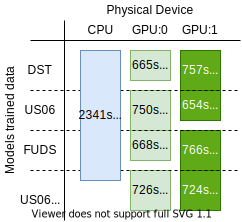
\includegraphics[width=0.60\linewidth]{II_Body/images/Accuracy_Compute.png}
    % \includesvg[width=\linewidth]{II_Body/images/Accuracy_Compute_10.svg}
    \caption{Accuracy computation using a single model trained on different proflies separately. The timing examples were taken from Model №5 computation process.}
    \label{fig:device_compute}
\end{figure}
\begin{table}[ht]
    \centering
    \caption{Model performance results across multiple devices..}
    \label{tab:speed}
    \begin{tabular}{c c c |c c c}
        \hline
        Structure                &Total params& flop/it & Coral TPU (ms) & R-Pi4 (ms)      & Android (ms) \\
        \hline
        1 $\times$ LSTM(500)     & 1,008,501  & 2.0G & 227.9$\pm$17.2 & 2021.6$\pm$164.9 & 4058.7$\pm$45.0 \\% 4048.0$\pm$69.0 \\   %FLOPs:2,018,005
        1 $\times$ GRU(560)      & 949,761    & 1.9G & 198.3$\pm$36.6 & 2104.2$\pm$109.6 & 3809.2$\pm$41.5 \\%3815.9$\pm$33.0 \\   %FLOPs:189,903
        LSTM(500) \& Atten
                                 & 1,361,881  & 3.2G & 206.9$\pm$32.9 & 2125.2$\pm$126.1 & 4711.2$\pm$51.0 \\%4711.8$\pm$41.5 \\ %FLOPs:3,222,344
%        2 $\times$ GRU(60)       & 33,762     & Unkn & ** & ** & \\
        1 $\times$ GRU(500)      & 758,001    & 1.5G & 140.8$\pm$24.7 & 1816.1$\pm$129.1 & 3227.5$\pm$37.5 \\%3241.7$\pm$32.5 \\  % FLOPs:1,516,503
        2 $\times$ LSTM(250)     & 504,201    & 1.1G & 102.2$\pm$16.3 & 1802.6$\pm$131.1 & 2494.4$\pm$34.0 \\%2454.4$\pm$33.0 \\   % FLOPs:1,109,409
%        1 $\times$ Layer \& Dense& 3,369      &     & 2.35$\pm$0.25  & 3.15$\pm$0.85 & 6.3*\\
        \hline
    \end{tabular}
\end{table}

\section{Conclusion} \label{sec:conclussion}
%* Summarise
%* -Testing approach
%* -Results
%* -Future work
%? Summarise key findings
%? - Accurate methods of developed to fit ML to SoC
%? - BEst training - Best model

%
%
The work has offered several implementations of Machine Learning algorithms for State of Charge estimation of A123 Lithium-Ion batteries.
Several Recursive Neural Network models were selected from already published based on the most common and promising structures and optimisers.
Five models were investigated, implemented, performance measured, and cross-evaluated using three drive cycles at five battery temperature ranges together from 20-50\textdegree{}.
Half a dozen thousand samples per profile of charge and discharge cycles were resampled to equal 1Hz rate and organised in 500 samples long matrices consisting of Voltage, Current, Temperature and corresponding charge percentage.
To adequately compare performance across models and comprehend the stochastic nature of Machine Learning a set of hyperparameters was predetermined through trial and error evaluation and multiple attempts of averaging.
By involving a learning rate scheduler and rollback technique to justify early stopping the speed of the training has been increased and the probability of model early overfill has been reduced.

%
%
After comparing 135 models of different sets of Layers and Neurons, the most accurate, lightweight and reasonable training time long ended up being 3 layers with 43 neurons per each.
Then, another 150 combinations of 5 methods models for 3 driving profiles ten times were processed through the same training, testing and performance measurement procedures, to conclude that a DST-based simple LSTM with Adam optimisers make the best self and others capturing model.
The next, which can closely match the same results, but with better self-capturing capabilities ended up being an LSTM with an Attention model.
While an Attention layer had a significant impact on capturing the complex driving profiles like FUDS, it failed to characterise the other two.
Both models were trained for relatively the same number of epochs, going through multiple attempts of learning rate reduction scheduler to achieve the lowest possible optimum.
Even though the error results were mostly commonly doubled from their already published equivalents, with the tripled amount of data and complexity of fitting both charge and discharge cycles, the increased error in prediction battery cycles remained below 5\% and line fitting accurately describes a State of Charge behaviour, especially at critical points of full charge and depletion.

%
%
Even though most models provided excellent results, they lacked the accuracy of time-series models, observed in similar scenarios.
The highest error regions were observed at the middle point of the charge, where the voltage of Lithium Ion batteries stays at 3.3V most of the time.
Being the SoC the function of current, that behaviour could indicate that Recurrent Neural Networks are tended to put more weight on the voltage feature instead.
While Model \#1 was chosen to be the best model for generalisation driving behaviour, it has little room for improvement, whereas Model \#3 with its extension to the structure may prove as a vital starting point for the next research iteration of charge prediction models, utilising output feature as an input, like time-series models tend to do in the other scenarios.

\section{Acknowledgements}\label{sec:acknowledgements}
The research was undertaken through funding from the Automotive Engineering Graduate Program (AEGP) in cooperation with the Queensland government and Prohelion industry partner.
All models evaluation has been performed through the help of the QUT HDR research and technical staff, who arranged access to the Hight Performance Machine (HPC Lyra) for the extensive initial computations.
The research has been conducted in cooperation with Mr Sam Haines, who performed a similar investigation on a similar dataset using Kalman filters and its' branches.
In addition, both Sam and I owe our progress to our Principal and Associate supervisors, Associate Professors David Holmes and Geoff Walker, who have been following our progress through the entire research.
Finally, we gratefully acknowledge the original developers of the Machine Learning framework Tensorflow from Google, who wrote detailed guides and documentation for all necessary tools used throughout the investigation.
%It is worth acknowledging the input from Dr Olga, Dr Mahsa and Pr Lovell who showed a practical interesr in the research and ... contribtution.



\bibliography{
    ../Z-References/References,
    I_Introduction/BibIntro,
    II_Body/BibRNN,
    II_Body/LSTM/BibLSTM,
    II_Body/GRU/BibGRU,
    II_Body/Optimisers/BibOpt.bib
}
\clearpage
\appendix
\section{Appendix A: Robust Adam implementation}  \label{app:RoAdam}
\input{../X-Appendix/AppendixE}
\clearpage
\section{Appendix B: Getting Number of Flops from TF2.4}  \label{app:flops}
\input{../X-Appendix/AppendixF}
\end{document}